% Options for packages loaded elsewhere
\PassOptionsToPackage{unicode}{hyperref}
\PassOptionsToPackage{hyphens}{url}
%
\documentclass[
  ignorenonframetext,
  aspectratio=169,
]{beamer}
\usepackage{pgfpages}
\setbeamertemplate{caption}[numbered]
\setbeamertemplate{caption label separator}{: }
\setbeamercolor{caption name}{fg=normal text.fg}
\beamertemplatenavigationsymbolshorizontal
% Prevent slide breaks in the middle of a paragraph
\widowpenalties 1 10000
\raggedbottom
\setbeamertemplate{part page}{
  \centering
  \begin{beamercolorbox}[sep=16pt,center]{part title}
    \usebeamerfont{part title}\insertpart\par
  \end{beamercolorbox}
}
\setbeamertemplate{section page}{
  \centering
  \begin{beamercolorbox}[sep=12pt,center]{section title}
    \usebeamerfont{section title}\insertsection\par
  \end{beamercolorbox}
}
\setbeamertemplate{subsection page}{
  \centering
  \begin{beamercolorbox}[sep=8pt,center]{subsection title}
    \usebeamerfont{subsection title}\insertsubsection\par
  \end{beamercolorbox}
}
\AtBeginPart{
  \frame{\partpage}
}
\AtBeginSection{
  \ifbibliography
  \else
    \frame{\sectionpage}
  \fi
}
\AtBeginSubsection{
  \frame{\subsectionpage}
}

\usepackage{amsmath,amssymb}
\usepackage{iftex}
\ifPDFTeX
  \usepackage[T1]{fontenc}
  \usepackage[utf8]{inputenc}
  \usepackage{textcomp} % provide euro and other symbols
\else % if luatex or xetex
  \usepackage{unicode-math}
  \defaultfontfeatures{Scale=MatchLowercase}
  \defaultfontfeatures[\rmfamily]{Ligatures=TeX,Scale=1}
\fi
\usepackage{lmodern}
\usetheme[]{techroom/pp.scss}
\ifPDFTeX\else  
    % xetex/luatex font selection
\fi
% Use upquote if available, for straight quotes in verbatim environments
\IfFileExists{upquote.sty}{\usepackage{upquote}}{}
\IfFileExists{microtype.sty}{% use microtype if available
  \usepackage[]{microtype}
  \UseMicrotypeSet[protrusion]{basicmath} % disable protrusion for tt fonts
}{}
\makeatletter
\@ifundefined{KOMAClassName}{% if non-KOMA class
  \IfFileExists{parskip.sty}{%
    \usepackage{parskip}
  }{% else
    \setlength{\parindent}{0pt}
    \setlength{\parskip}{6pt plus 2pt minus 1pt}}
}{% if KOMA class
  \KOMAoptions{parskip=half}}
\makeatother
\usepackage{xcolor}
\newif\ifbibliography
\setlength{\emergencystretch}{3em} % prevent overfull lines
\setcounter{secnumdepth}{-\maxdimen} % remove section numbering


\providecommand{\tightlist}{%
  \setlength{\itemsep}{0pt}\setlength{\parskip}{0pt}}\usepackage{longtable,booktabs,array}
\usepackage{calc} % for calculating minipage widths
\usepackage{caption}
% Make caption package work with longtable
\makeatletter
\def\fnum@table{\tablename~\thetable}
\makeatother
\usepackage{graphicx}
\makeatletter
\newsavebox\pandoc@box
\newcommand*\pandocbounded[1]{% scales image to fit in text height/width
  \sbox\pandoc@box{#1}%
  \Gscale@div\@tempa{\textheight}{\dimexpr\ht\pandoc@box+\dp\pandoc@box\relax}%
  \Gscale@div\@tempb{\linewidth}{\wd\pandoc@box}%
  \ifdim\@tempb\p@<\@tempa\p@\let\@tempa\@tempb\fi% select the smaller of both
  \ifdim\@tempa\p@<\p@\scalebox{\@tempa}{\usebox\pandoc@box}%
  \else\usebox{\pandoc@box}%
  \fi%
}
% Set default figure placement to htbp
\def\fps@figure{htbp}
\makeatother

\makeatletter
\@ifpackageloaded{caption}{}{\usepackage{caption}}
\AtBeginDocument{%
\ifdefined\contentsname
  \renewcommand*\contentsname{Table of contents}
\else
  \newcommand\contentsname{Table of contents}
\fi
\ifdefined\listfigurename
  \renewcommand*\listfigurename{List of Figures}
\else
  \newcommand\listfigurename{List of Figures}
\fi
\ifdefined\listtablename
  \renewcommand*\listtablename{List of Tables}
\else
  \newcommand\listtablename{List of Tables}
\fi
\ifdefined\figurename
  \renewcommand*\figurename{Figure}
\else
  \newcommand\figurename{Figure}
\fi
\ifdefined\tablename
  \renewcommand*\tablename{Table}
\else
  \newcommand\tablename{Table}
\fi
}
\@ifpackageloaded{float}{}{\usepackage{float}}
\floatstyle{ruled}
\@ifundefined{c@chapter}{\newfloat{codelisting}{h}{lop}}{\newfloat{codelisting}{h}{lop}[chapter]}
\floatname{codelisting}{Listing}
\newcommand*\listoflistings{\listof{codelisting}{List of Listings}}
\makeatother
\makeatletter
\makeatother
\makeatletter
\@ifpackageloaded{caption}{}{\usepackage{caption}}
\@ifpackageloaded{subcaption}{}{\usepackage{subcaption}}
\makeatother

\usepackage{bookmark}

\IfFileExists{xurl.sty}{\usepackage{xurl}}{} % add URL line breaks if available
\urlstyle{same} % disable monospaced font for URLs
\hypersetup{
  hidelinks,
  pdfcreator={LaTeX via pandoc}}


\author{}
\date{}
\logo{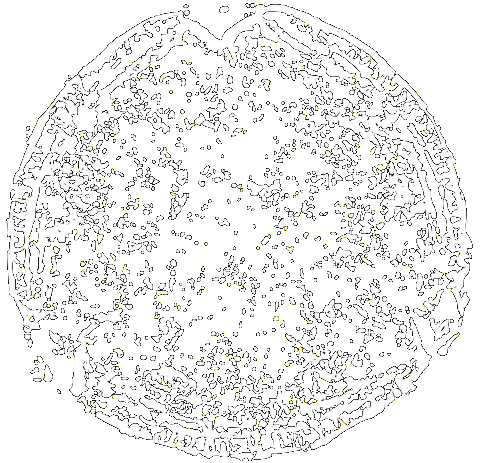
\includegraphics{images/pyl.png}}

\begin{document}


\begin{frame}{}
\phantomsection\label{section}
Pollen deposition on \emph{Succisa pratensis} in a dynamic
plant-pollinator network Jakub Štenc


\includegraphics[width=2.60417in,height=\textheight,keepaspectratio]{images/CREAF-SO-logo-pluma_blanca-ESP.png}


\includegraphics[width=1.91667in,height=\textheight,keepaspectratio]{images/logoPrF1.png}
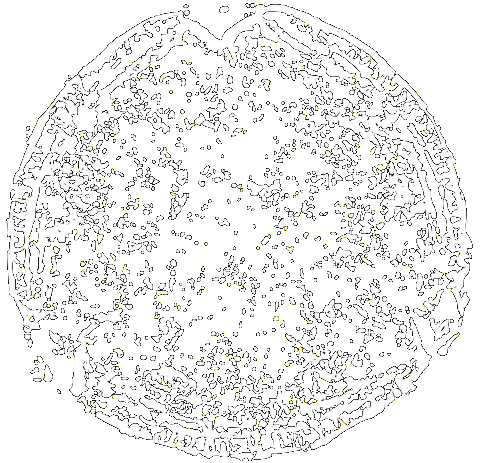
\includegraphics[width=1.91667in,height=\textheight,keepaspectratio]{images/pyl.png}

\begin{block}{Intro}
\phantomsection\label{intro}
\begin{justify}


\end{justify}

\begin{center}
\pandocbounded{\includegraphics[keepaspectratio]{images/video_intro_reduced.mp4}}
\end{center}
\end{block}

\begin{block}{Intro}
\phantomsection\label{intro-1}
\begin{center}
\pandocbounded{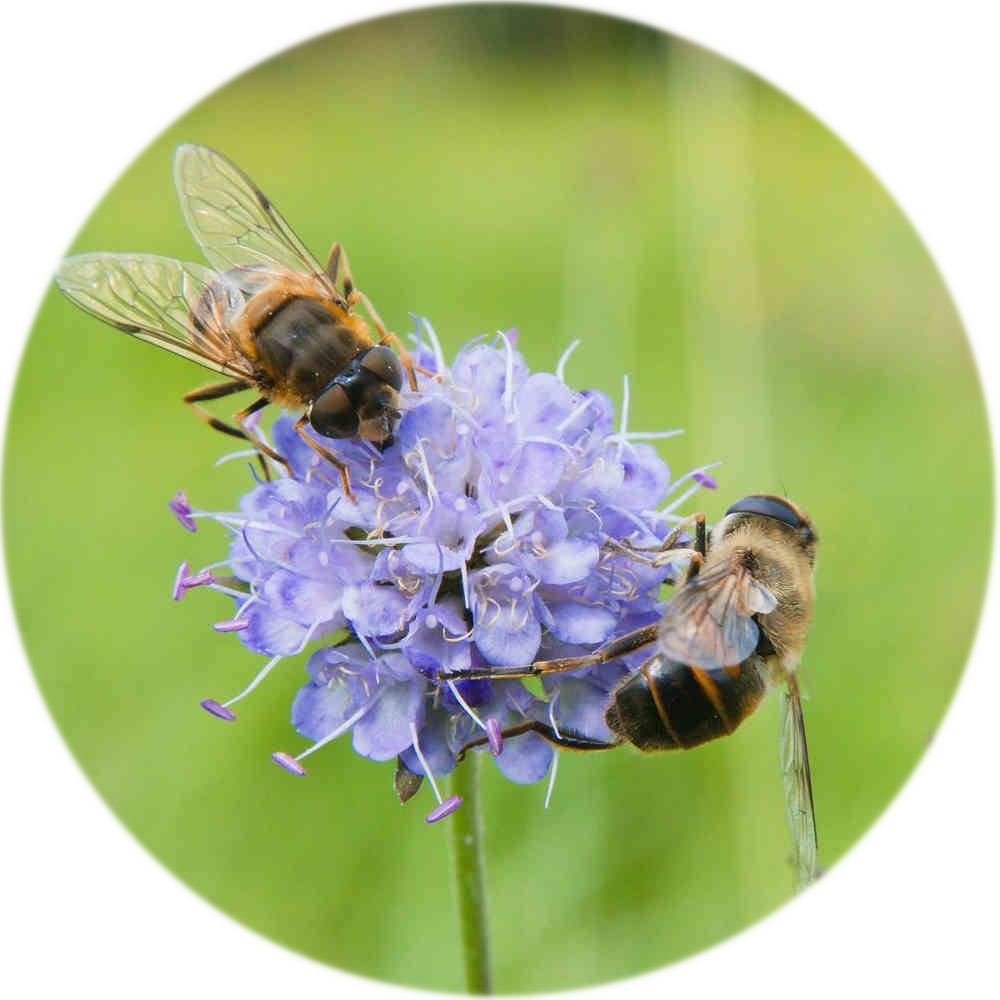
\includegraphics[keepaspectratio]{images/pestrenky_round.png}}
\end{center}
\end{block}

\begin{block}{Intro}
\phantomsection\label{intro-2}
\begin{center}
\pandocbounded{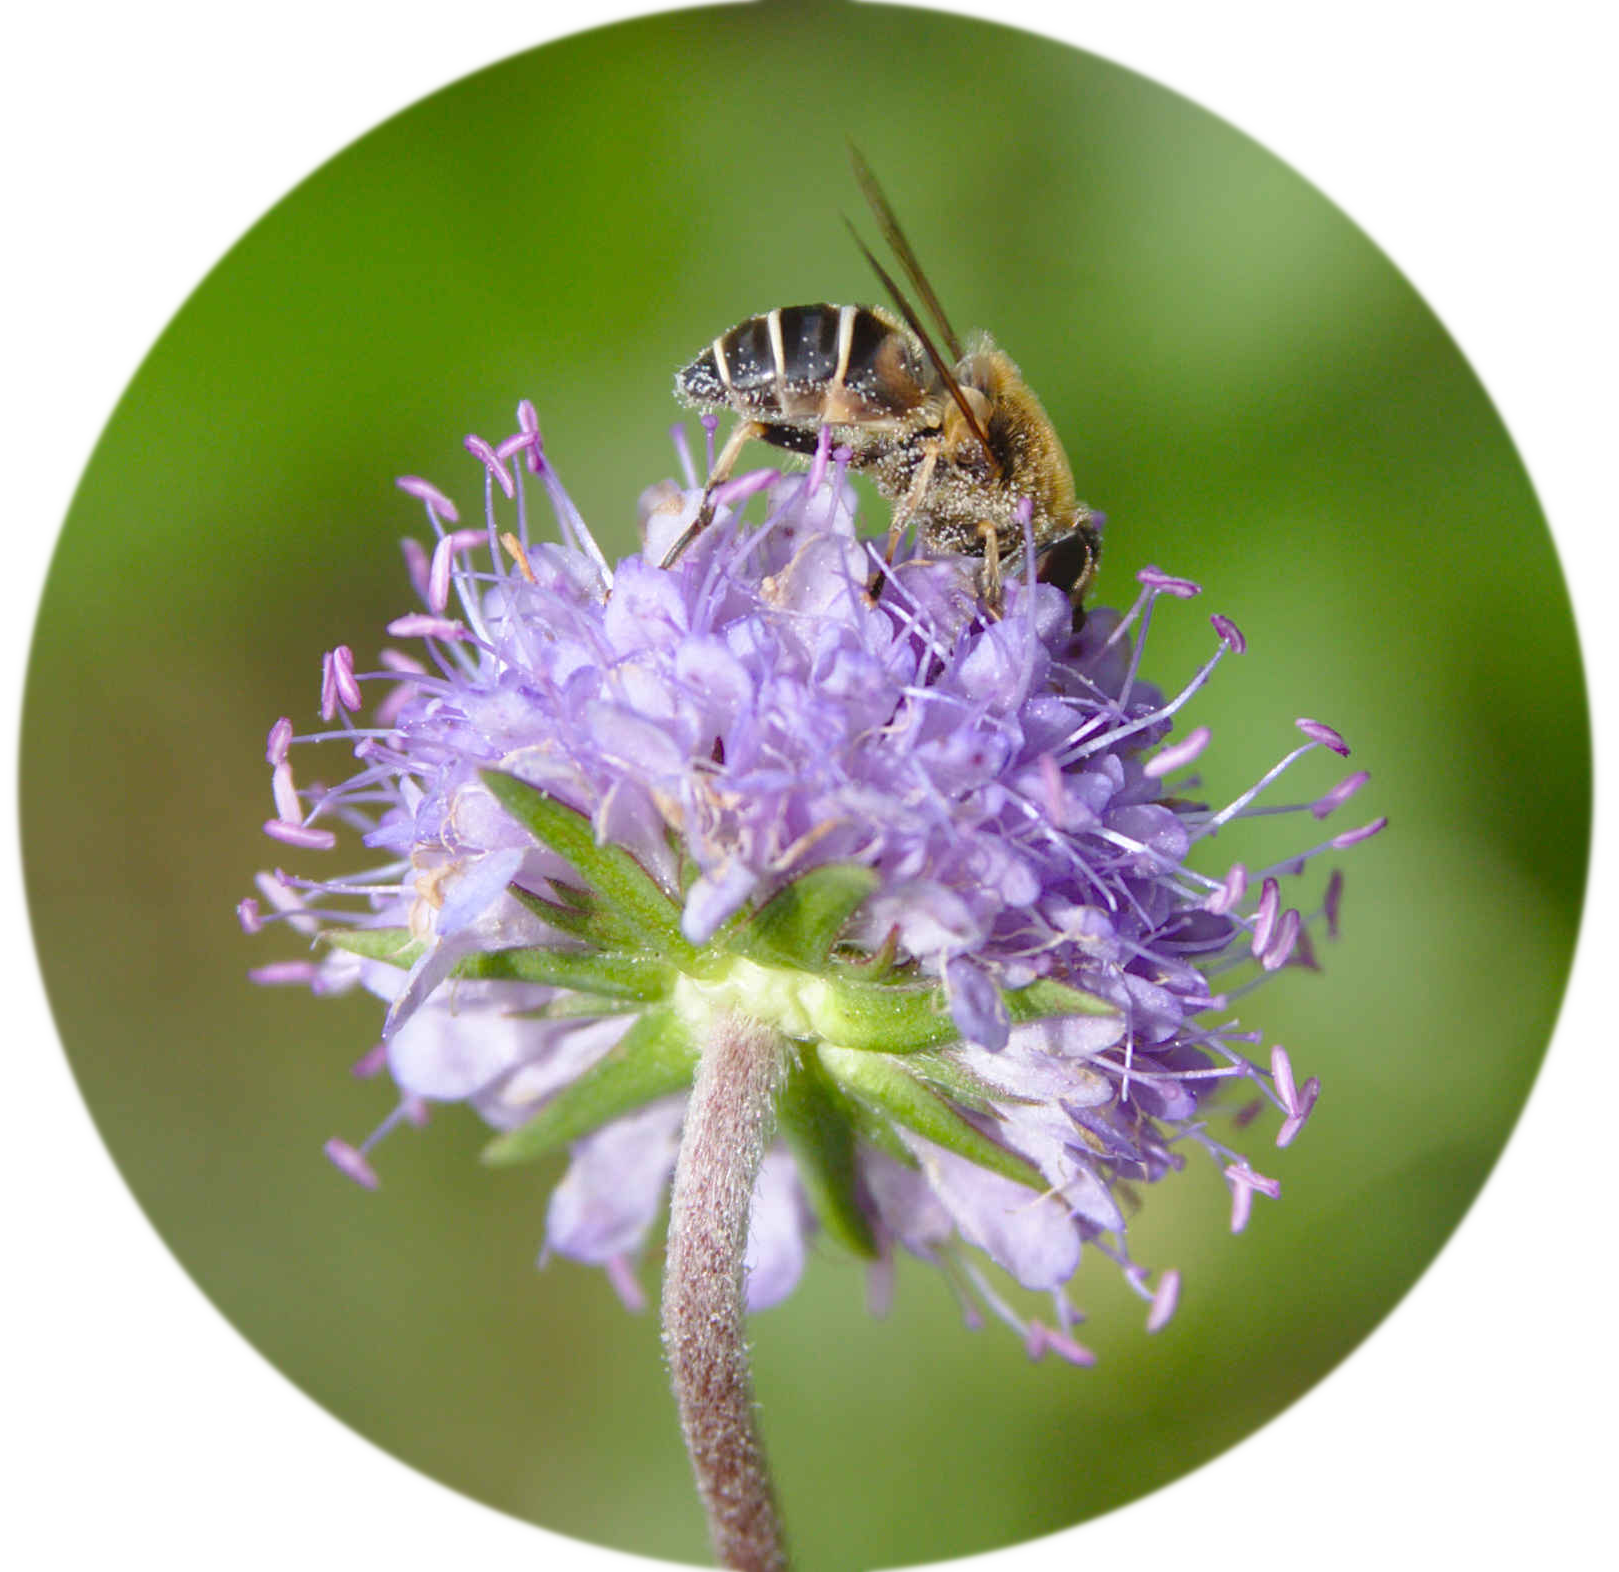
\includegraphics[keepaspectratio]{images/E.interuptus_round.png}}
\end{center}
\end{block}

\begin{block}{Intro}
\phantomsection\label{intro-3}
\begin{center}
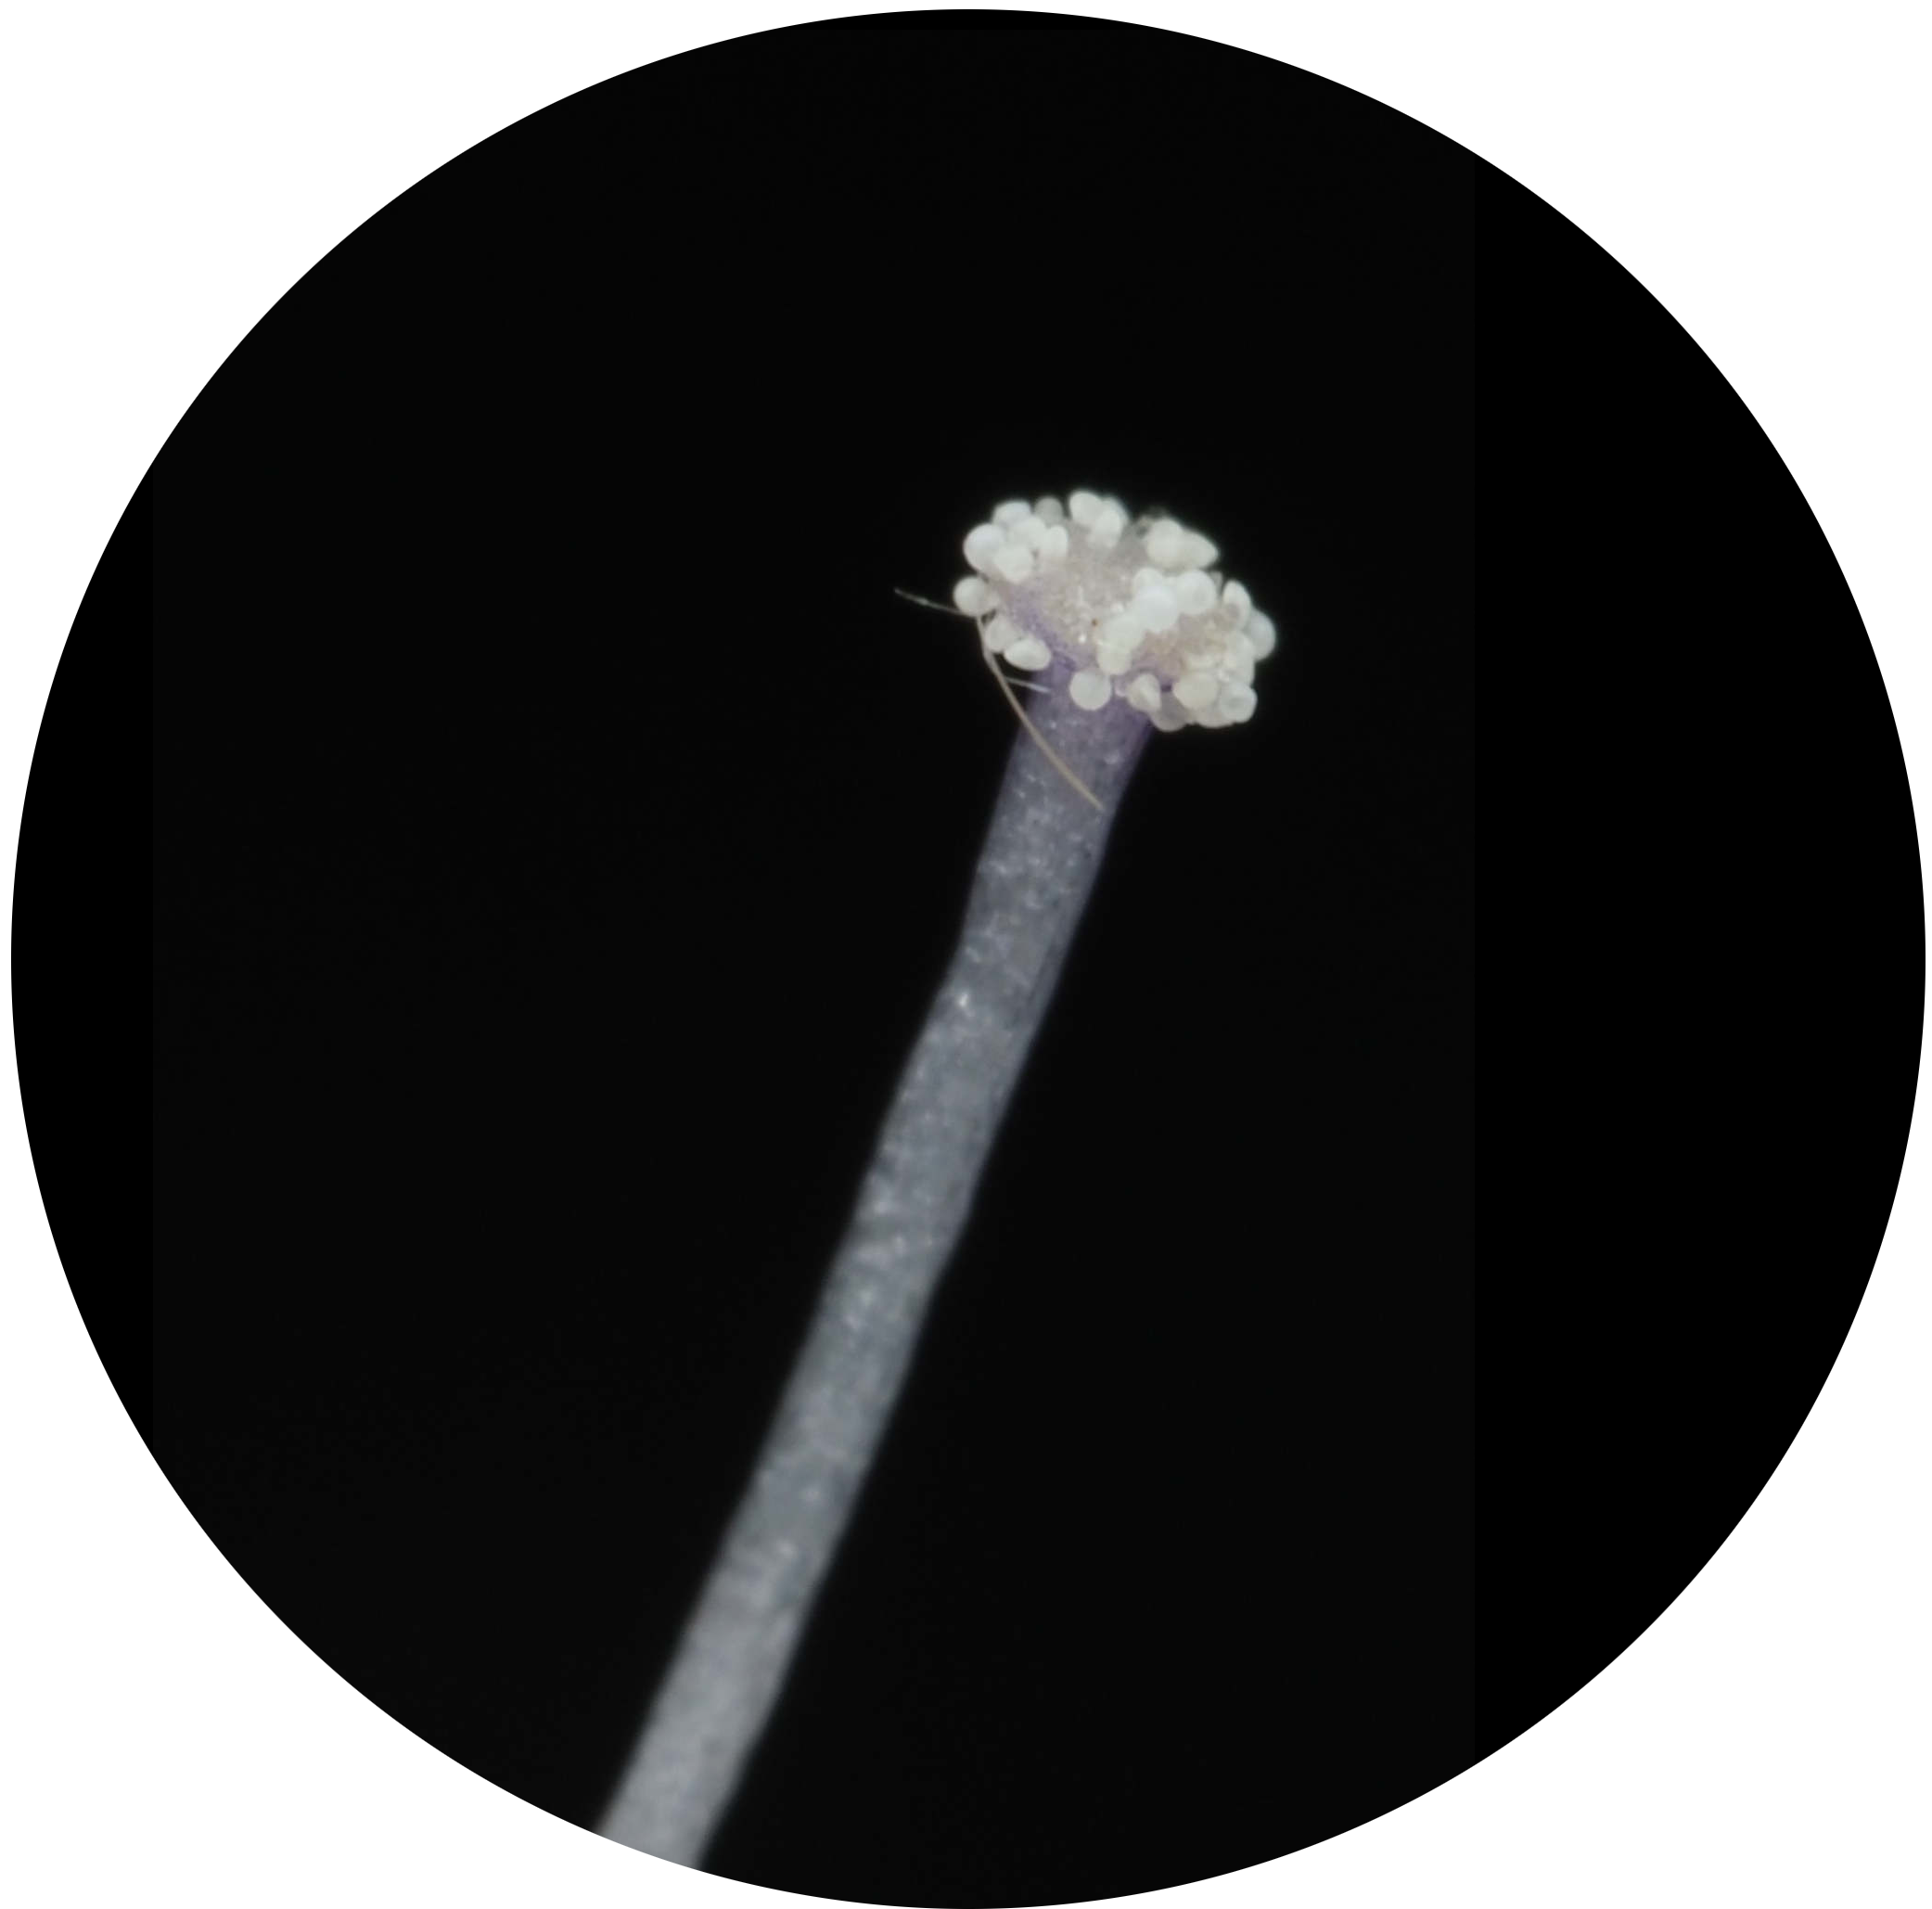
\includegraphics[width=2.53125in,height=\textheight,keepaspectratio]{images/stigma.png}
\end{center}
\end{block}

\begin{block}{Intro}
\phantomsection\label{intro-4}
\begin{center}
\pandocbounded{\includegraphics[keepaspectratio]{images/Blizna_Suc_pra_2_round.png}}
\end{center}
\end{block}

\begin{block}{Methods - the locality}
\phantomsection\label{methods---the-locality}
\begin{figure}

\begin{minipage}{0.50\linewidth}

\begin{figure}[H]

\subcaption{{Czech Republic}}

{\centering 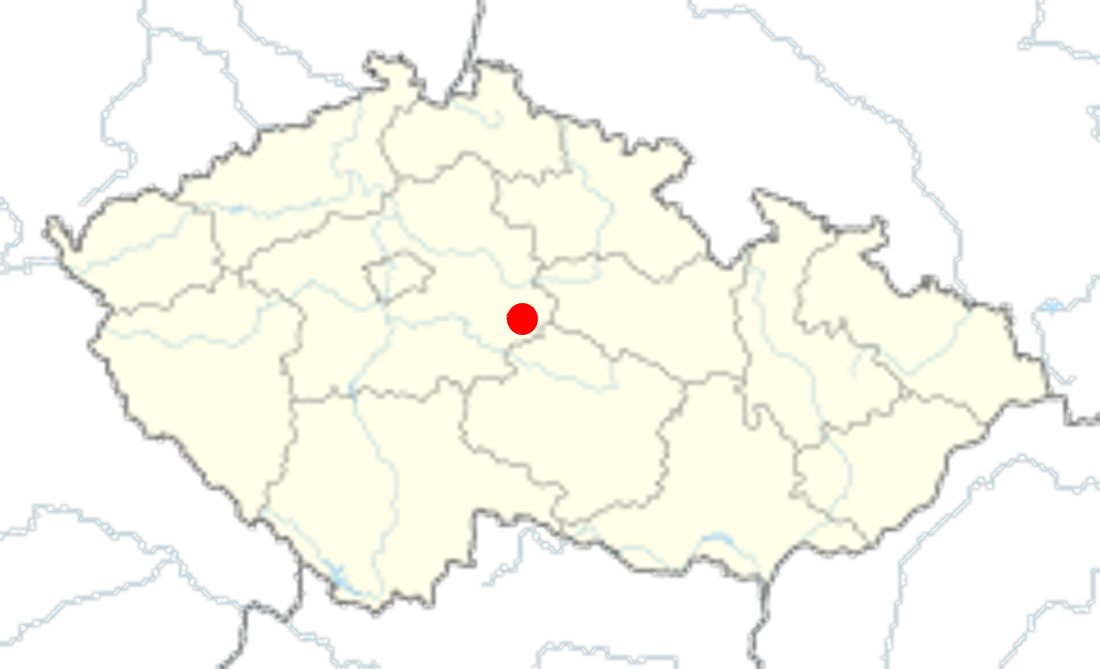
\includegraphics[width=4.16667in,height=\textheight,keepaspectratio]{images/Picture9.png}

}

\end{figure}%

\end{minipage}%
%
\begin{minipage}{0.50\linewidth}

\begin{figure}[H]

\subcaption{{Rich in flowers}}

{\centering 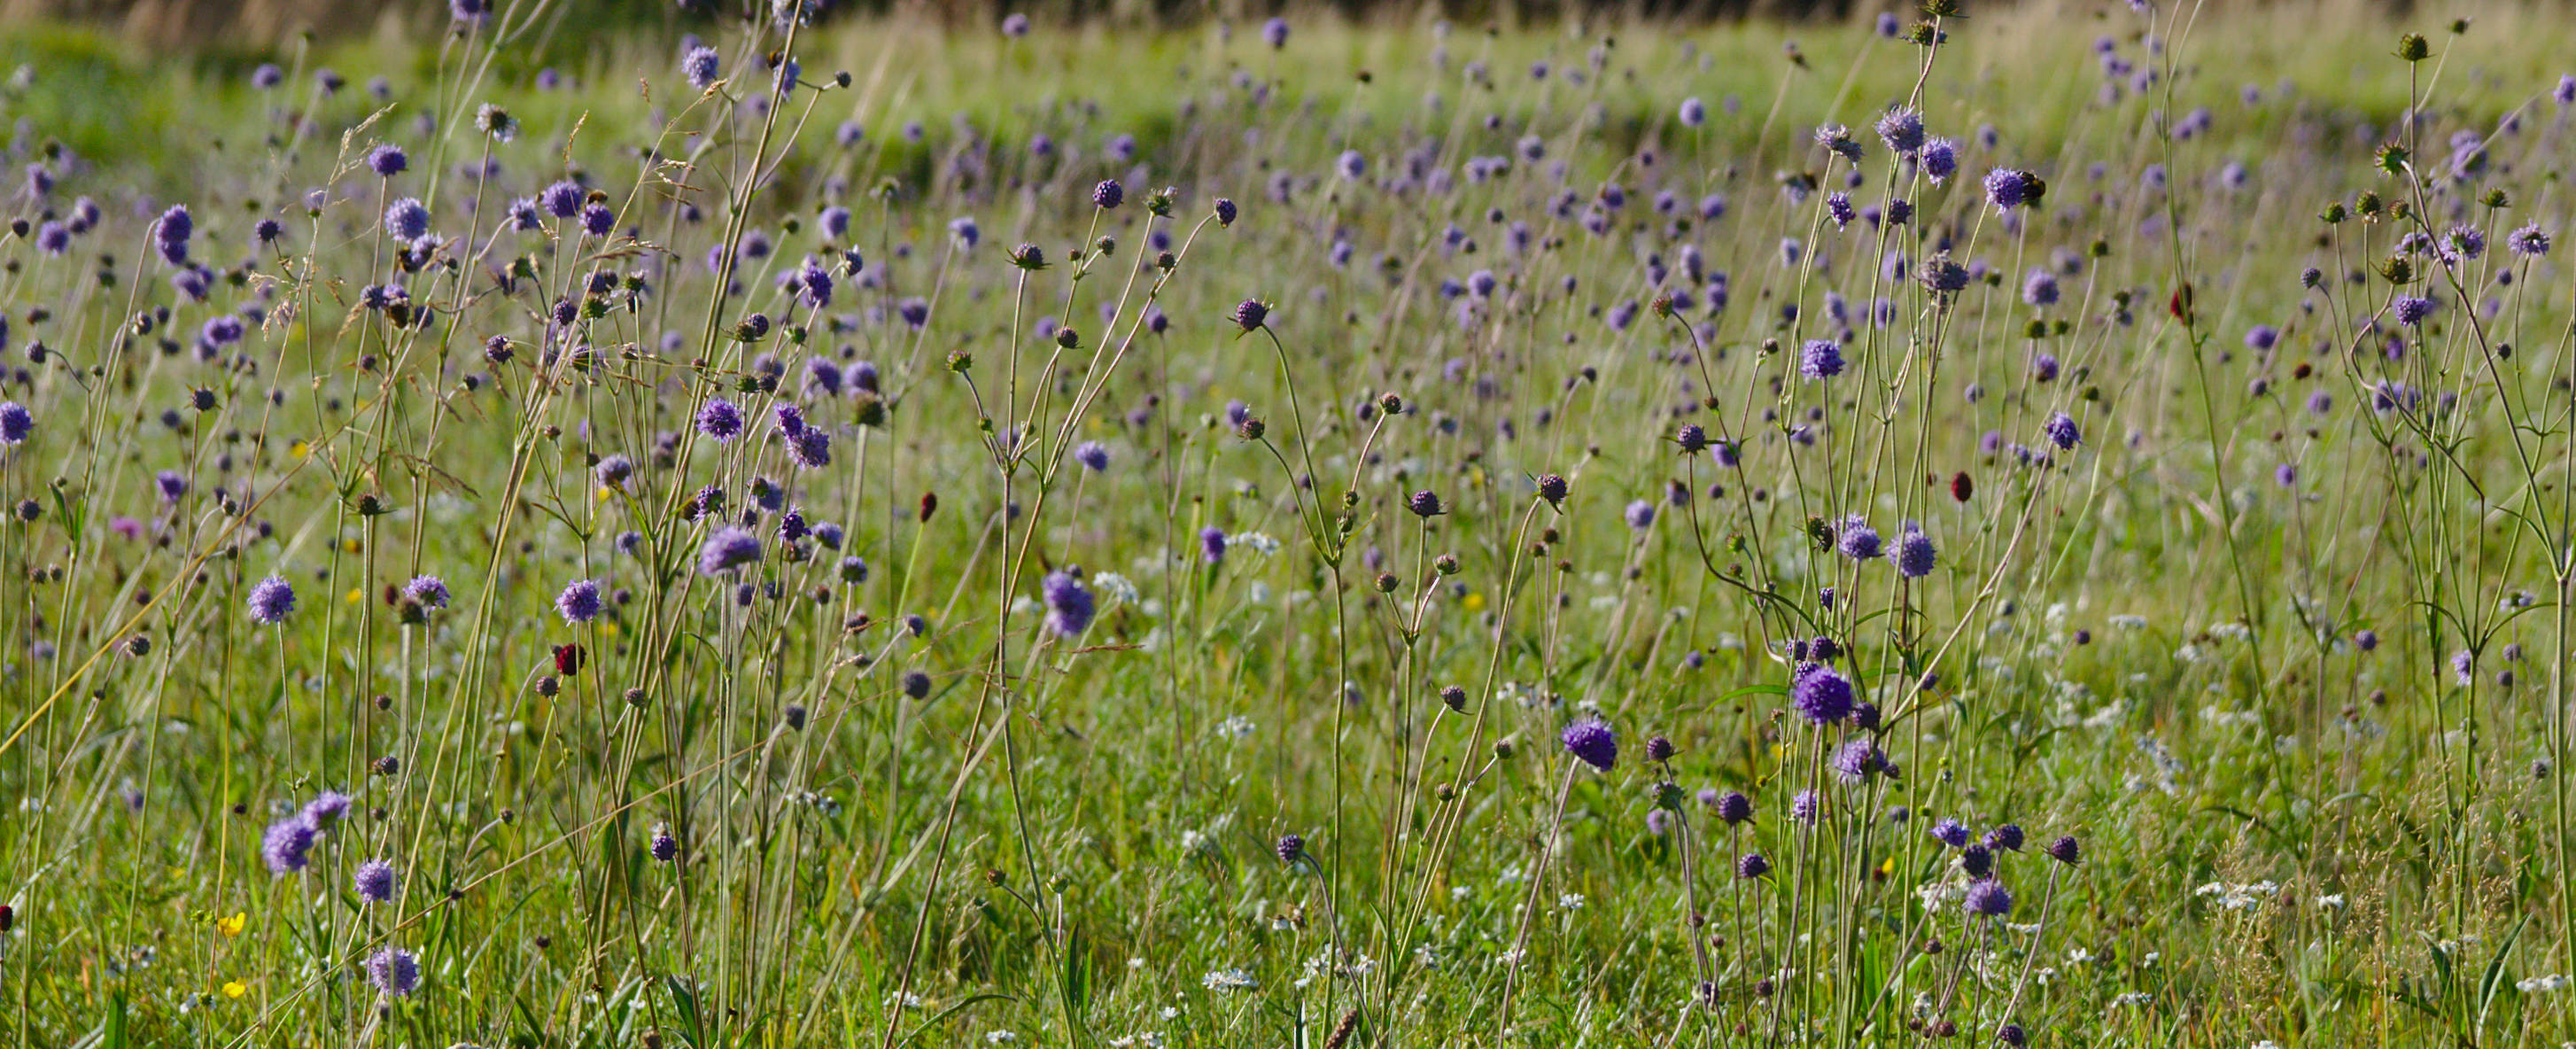
\includegraphics[width=8.33333in,height=\textheight,keepaspectratio]{images/banner.jpg}

}

\end{figure}%

\end{minipage}%

\end{figure}%

\begin{itemize}
\tightlist
\item
  15 years of data collection (2011-2025)
\end{itemize}
\end{block}

\begin{block}{Methods - permanent plots}
\phantomsection\label{methods---permanent-plots}
\begin{figure}

\begin{minipage}{0.33\linewidth}

\begin{figure}[H]

\subcaption{{plots are marked}}

{\centering 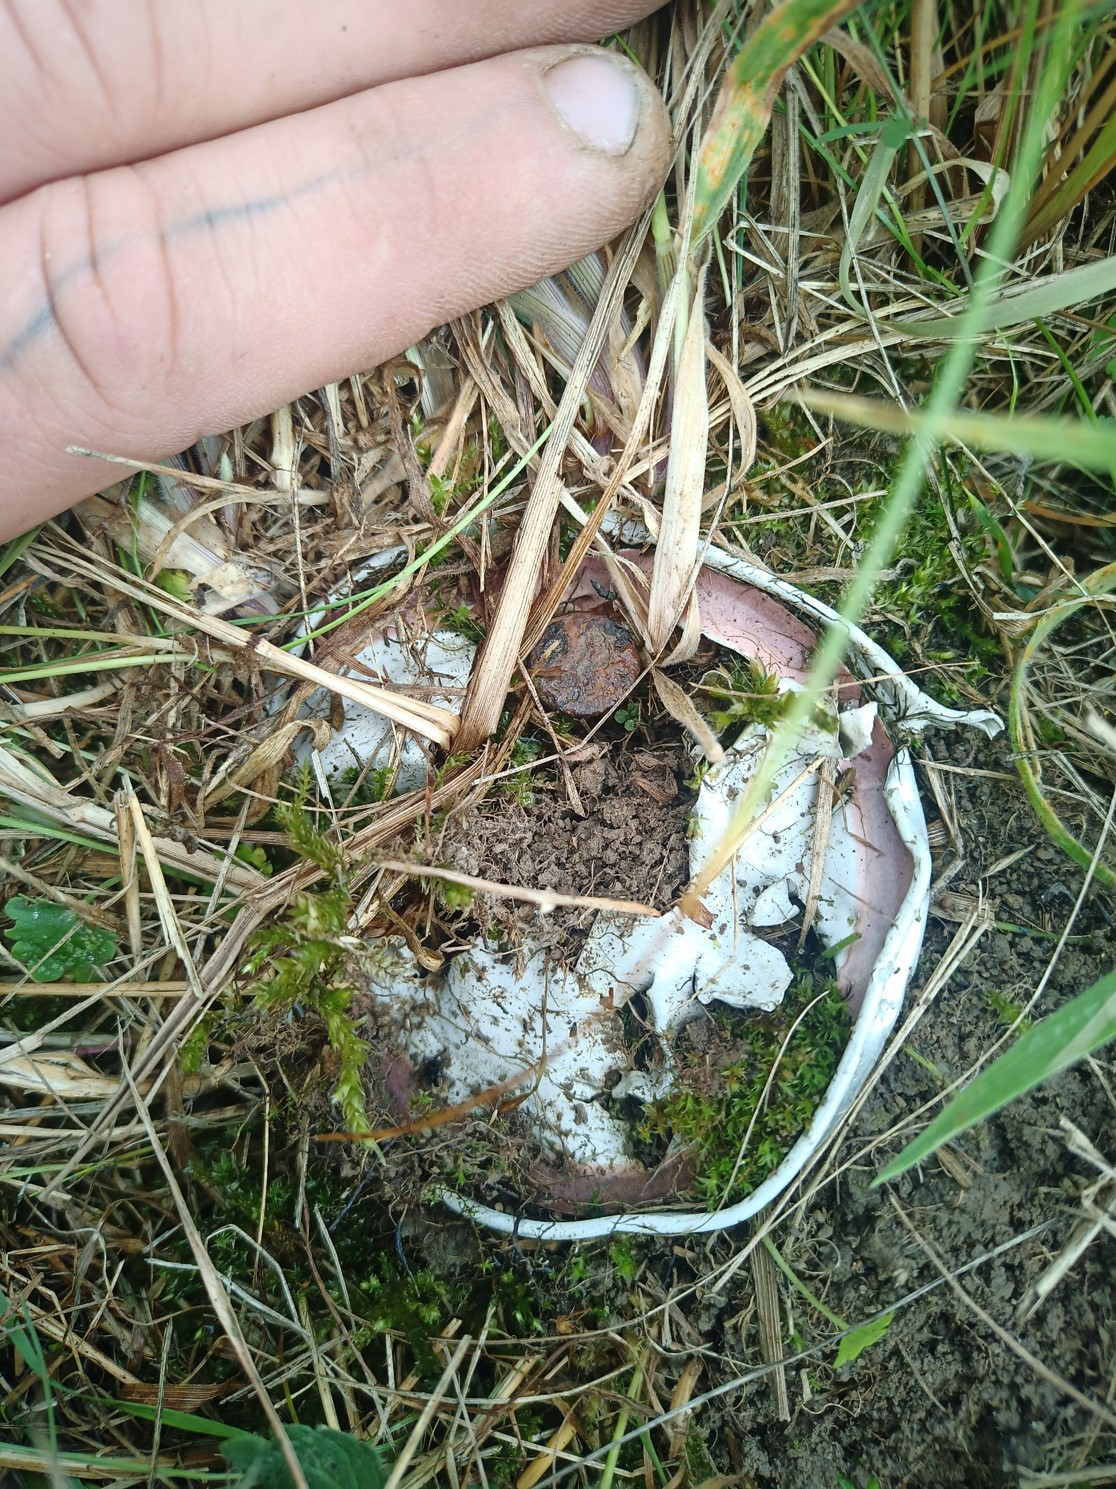
\includegraphics[width=3.125in,height=\textheight,keepaspectratio]{images/Picture3.jpg}

}

\end{figure}%

\end{minipage}%
%
\begin{minipage}{0.33\linewidth}

\begin{figure}[H]

\subcaption{{recovered every year}}

{\centering 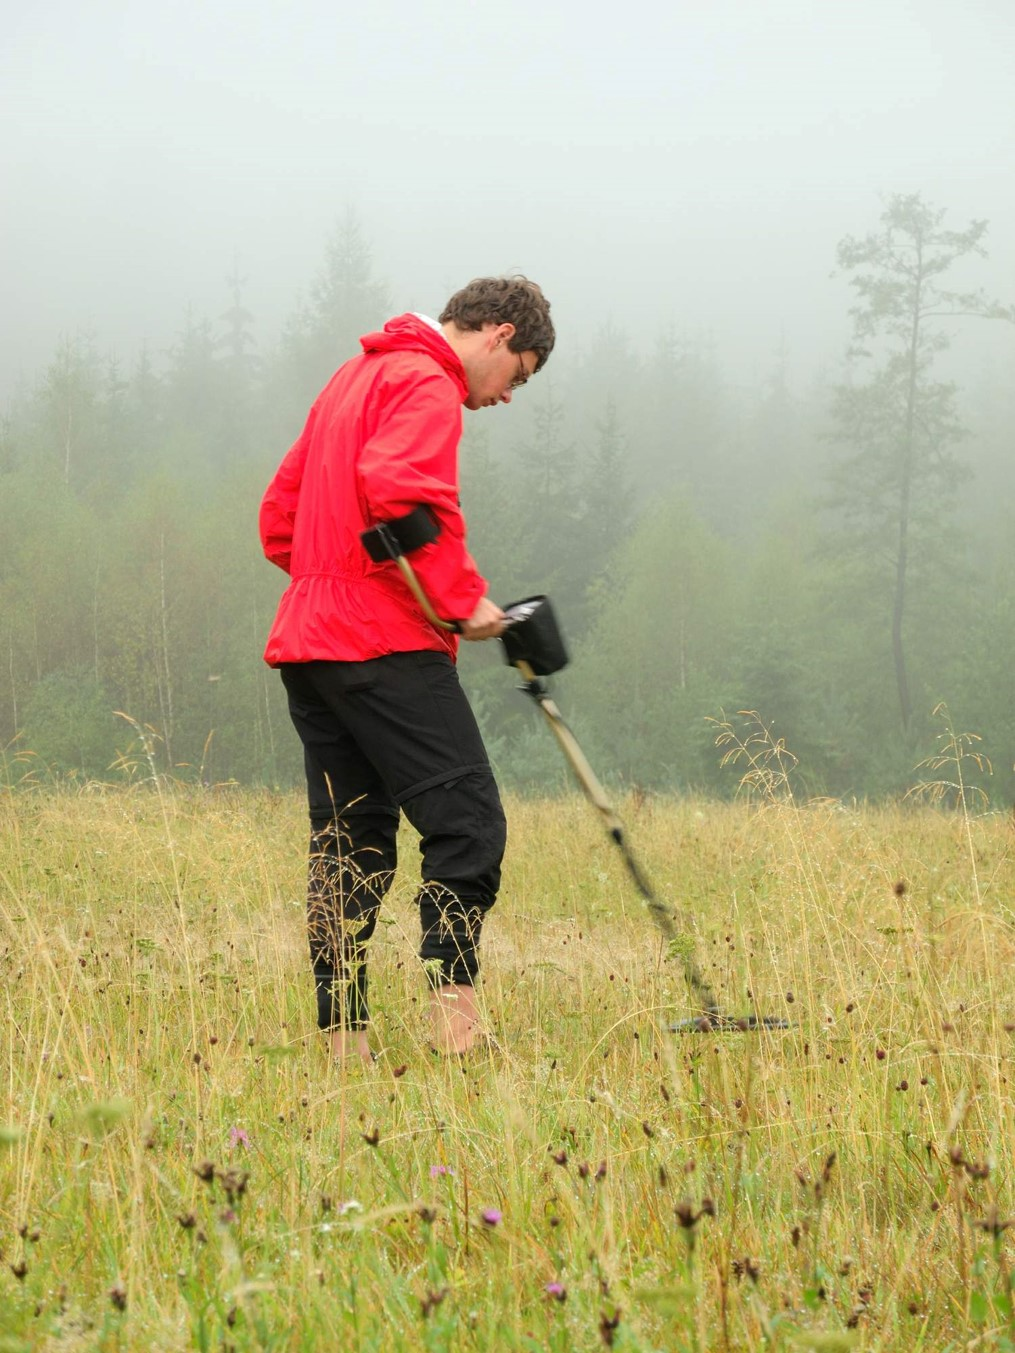
\includegraphics[width=3.125in,height=\textheight,keepaspectratio]{images/Picture2.jpg}

}

\end{figure}%

\end{minipage}%
%
\begin{minipage}{0.33\linewidth}

\begin{figure}[H]

\subcaption{{93 plots in total}}

{\centering \pandocbounded{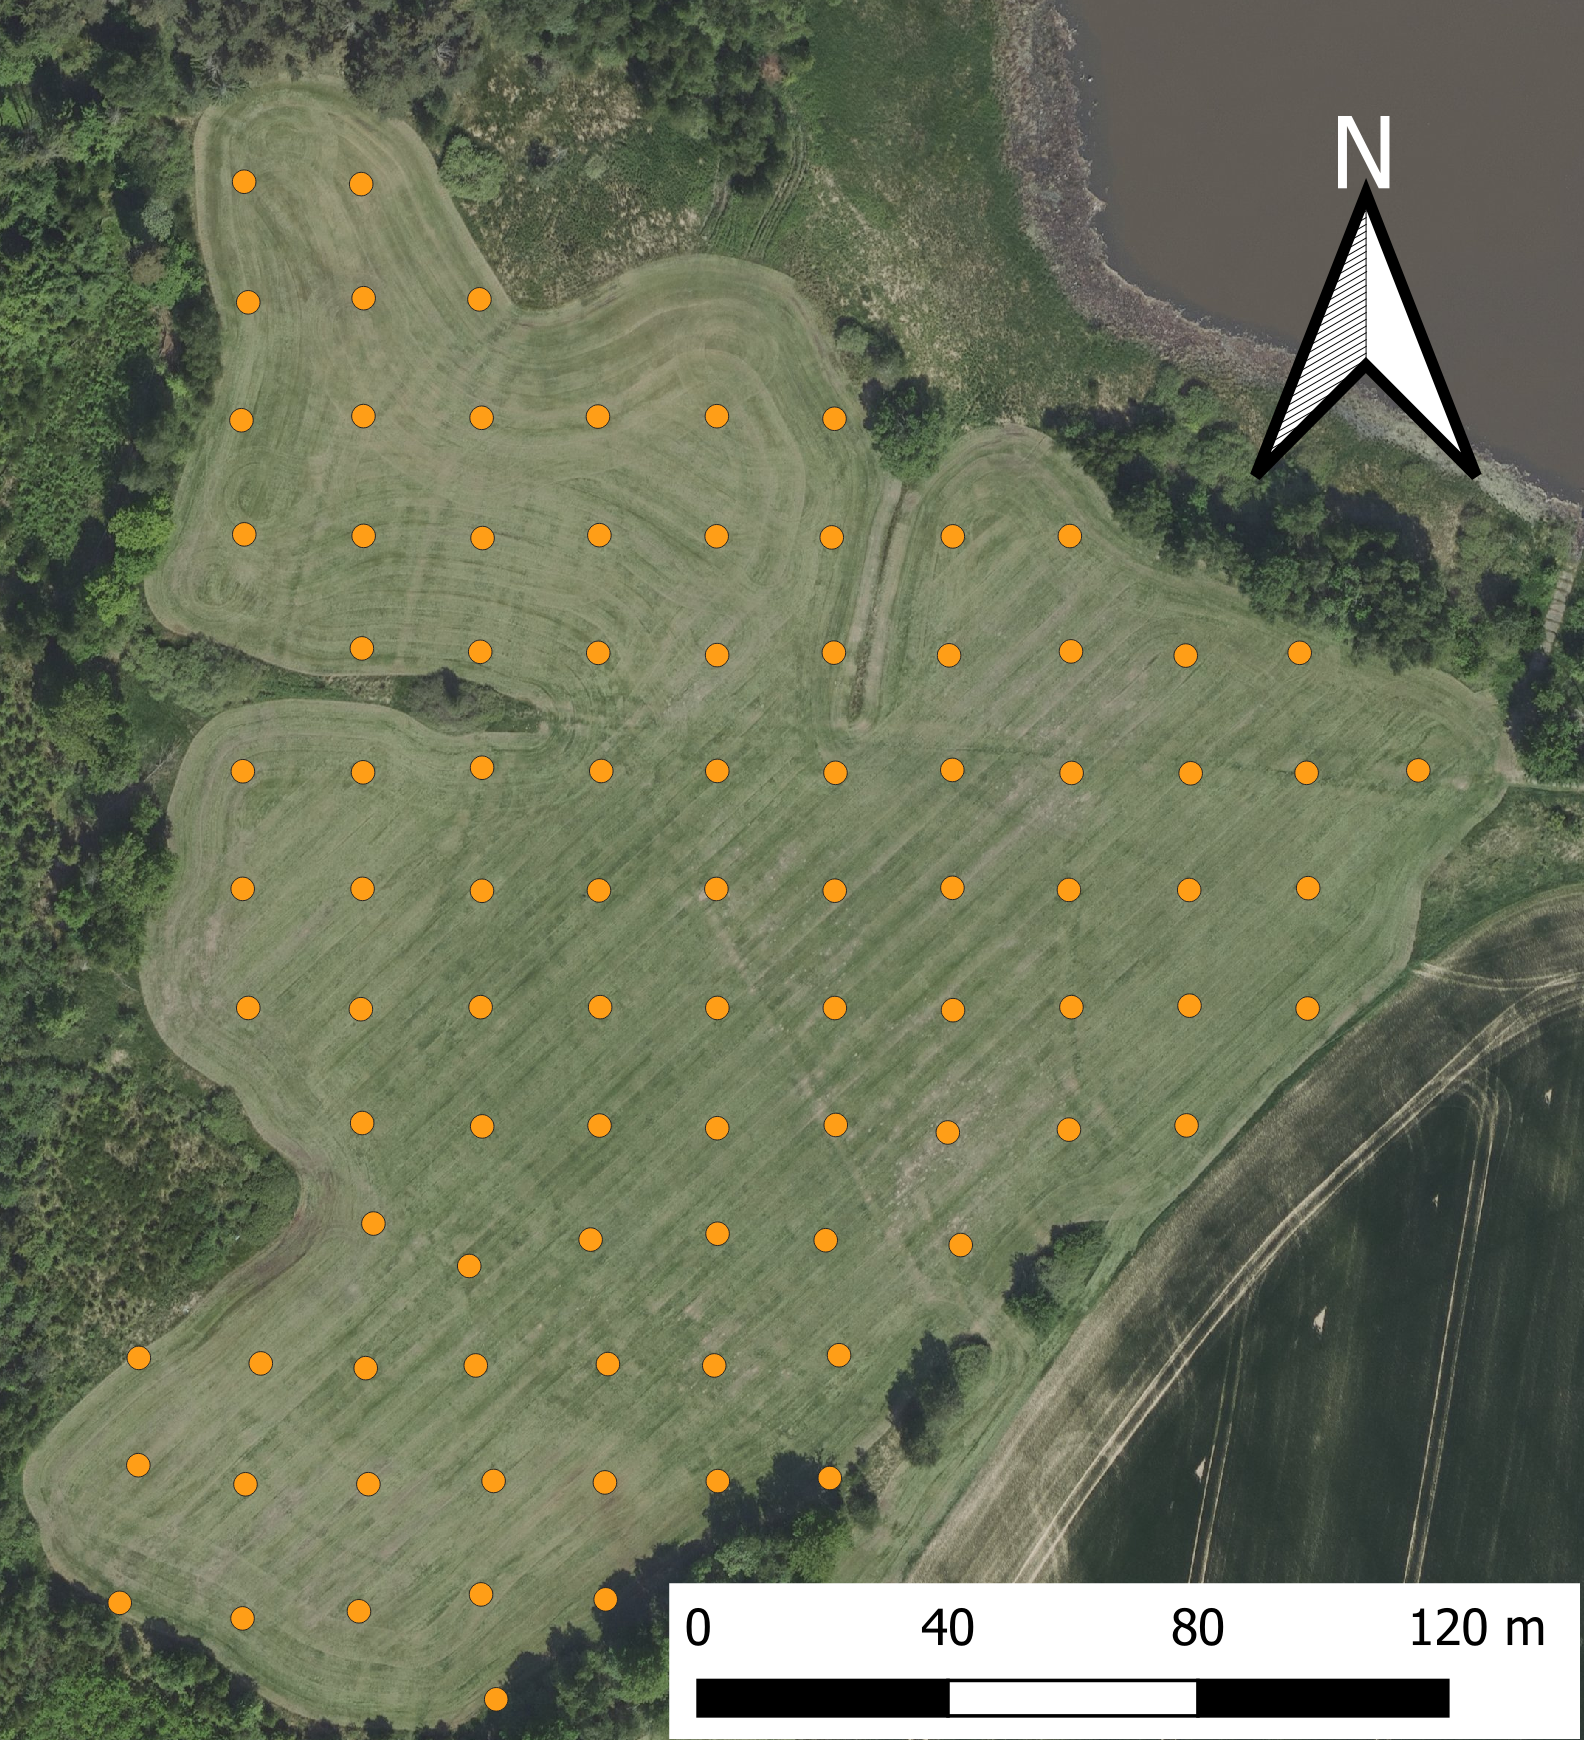
\includegraphics[keepaspectratio]{images/han_map_1.png}}

}

\end{figure}%

\end{minipage}%

\end{figure}%
\end{block}

\begin{block}{Methods - plant-pollinator survey}
\phantomsection\label{methods---plant-pollinator-survey}
\begin{figure}

\begin{minipage}{0.50\linewidth}

\begin{figure}[H]

\subcaption{{Plant survey}}

{\centering \pandocbounded{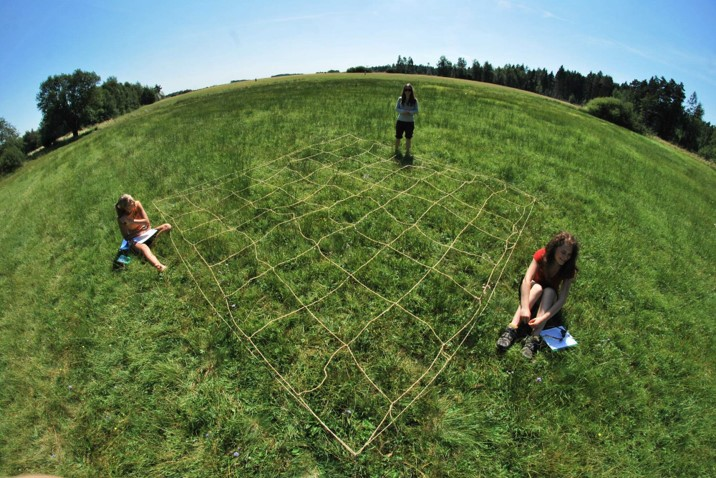
\includegraphics[keepaspectratio]{images/Picture1.jpg}}

}

\end{figure}%

\end{minipage}%
%
\begin{minipage}{0.50\linewidth}

\begin{figure}[H]

\subcaption{{Pollinator survey}}

{\centering \pandocbounded{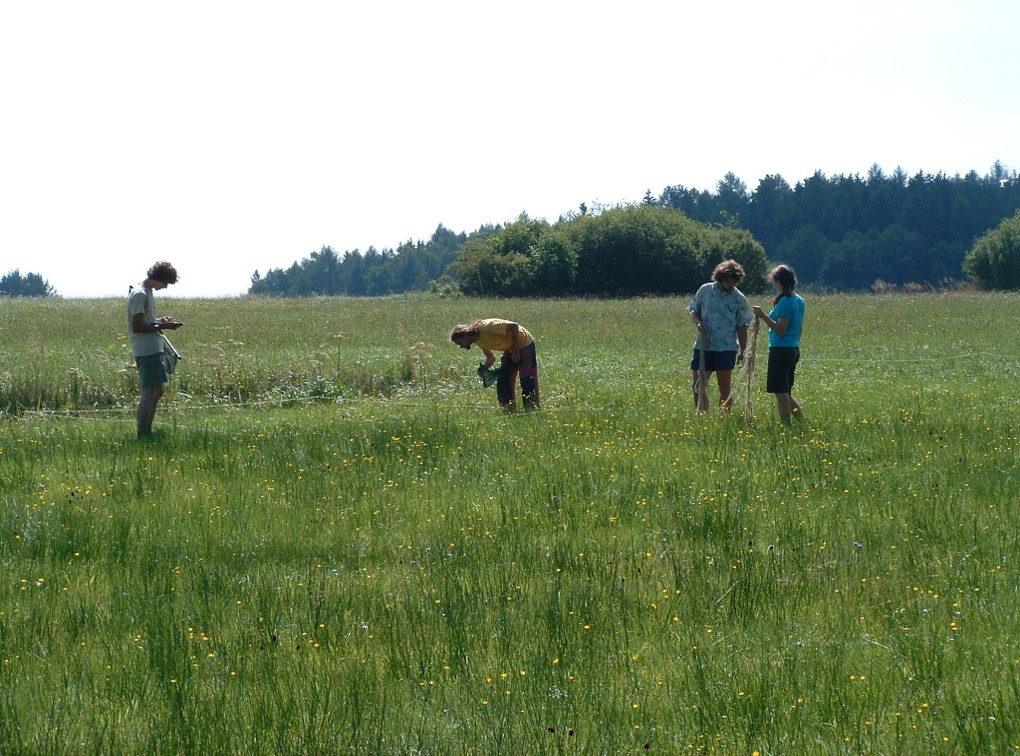
\includegraphics[keepaspectratio]{images/Picture5.jpg}}

}

\end{figure}%

\end{minipage}%

\end{figure}%
\end{block}

\begin{block}{Methods - plant survey}
\phantomsection\label{methods---plant-survey}
\begin{figure}

\begin{minipage}{0.50\linewidth}
\pandocbounded{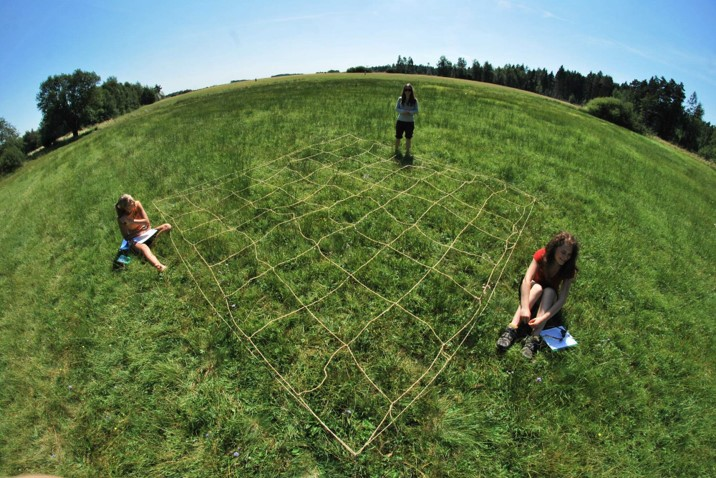
\includegraphics[keepaspectratio]{images/Picture1.jpg}}\end{minipage}%
%
\begin{minipage}{0.50\linewidth}

\end{minipage}%

\end{figure}%

\begin{itemize}
\tightlist
\item
  4 x 4 meter squares
\item
  divided to 64 0.5 x 0.5 subplots
\item
  Stalks of flowering plants are counted or scored presence/absence in
  subplots
\item
  2 times per sampling period
\end{itemize}
\end{block}

\begin{block}{Methods - pollinator survey}
\phantomsection\label{methods---pollinator-survey}
\begin{figure}

\begin{minipage}{0.50\linewidth}
\pandocbounded{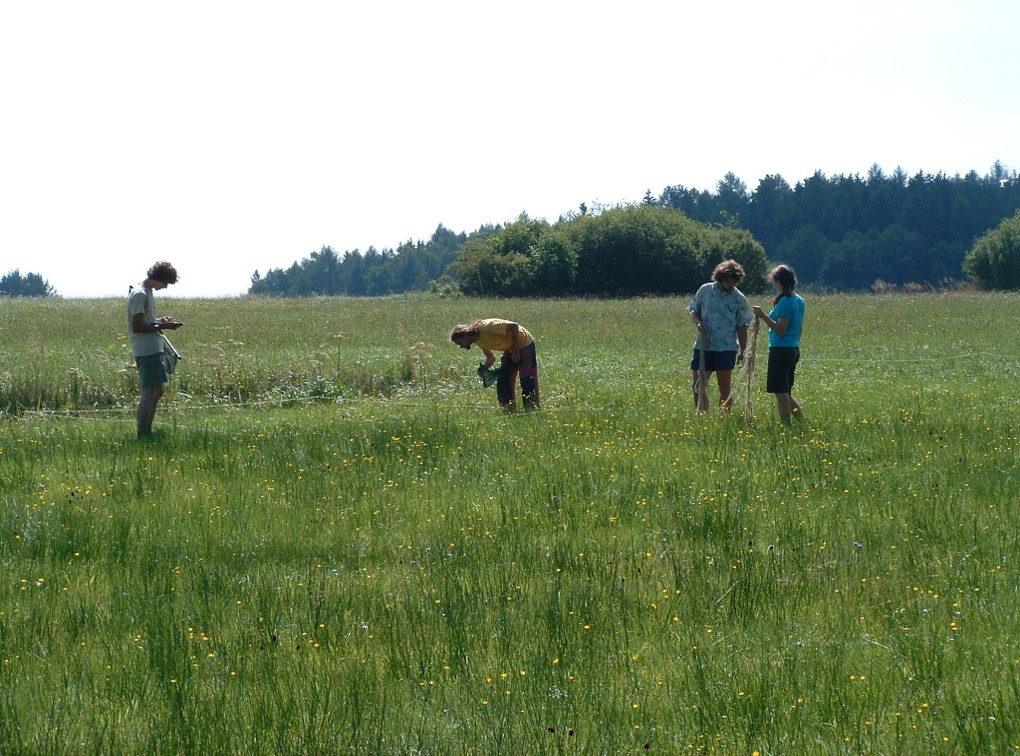
\includegraphics[keepaspectratio]{images/Picture5.jpg}}\end{minipage}%
%
\begin{minipage}{0.50\linewidth}

\end{minipage}%

\end{figure}%

\begin{itemize}
\tightlist
\item
  ``Snapshot'' of plant-pollinator interaction
\item
  = all interactions recorded, every flower unit observed once per
  sampling
\item
  20+ sampling per plot per year
\item
  97 629+ interactions recorded
\end{itemize}
\end{block}

\begin{block}{Methods - pollinator survey}
\phantomsection\label{methods---pollinator-survey-1}
\end{block}

\begin{block}{Pollinator sharing among plants}
\phantomsection\label{pollinator-sharing-among-plants}
\begin{center}
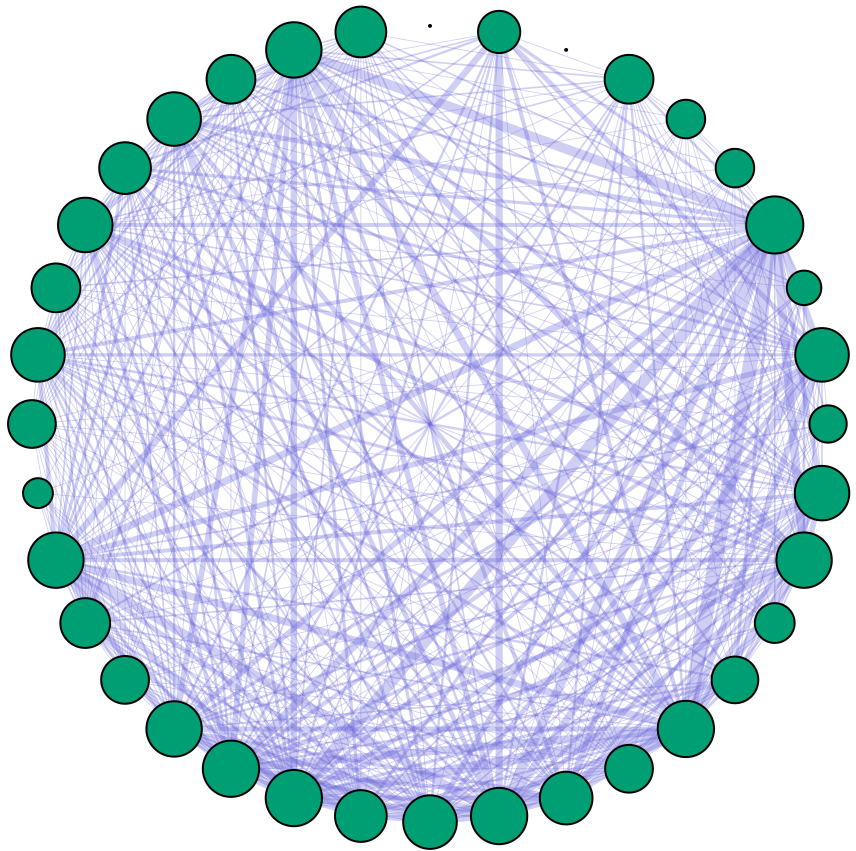
\includegraphics[width=2.5in,height=\textheight,keepaspectratio]{images/unnamed-chunk-4-1.png}
\end{center}
\end{block}

\begin{block}{Annual variation in pollinator sharing}
\phantomsection\label{annual-variation-in-pollinator-sharing}
\begin{figure}

\begin{minipage}{0.95\linewidth}
\begin{center}
\pandocbounded{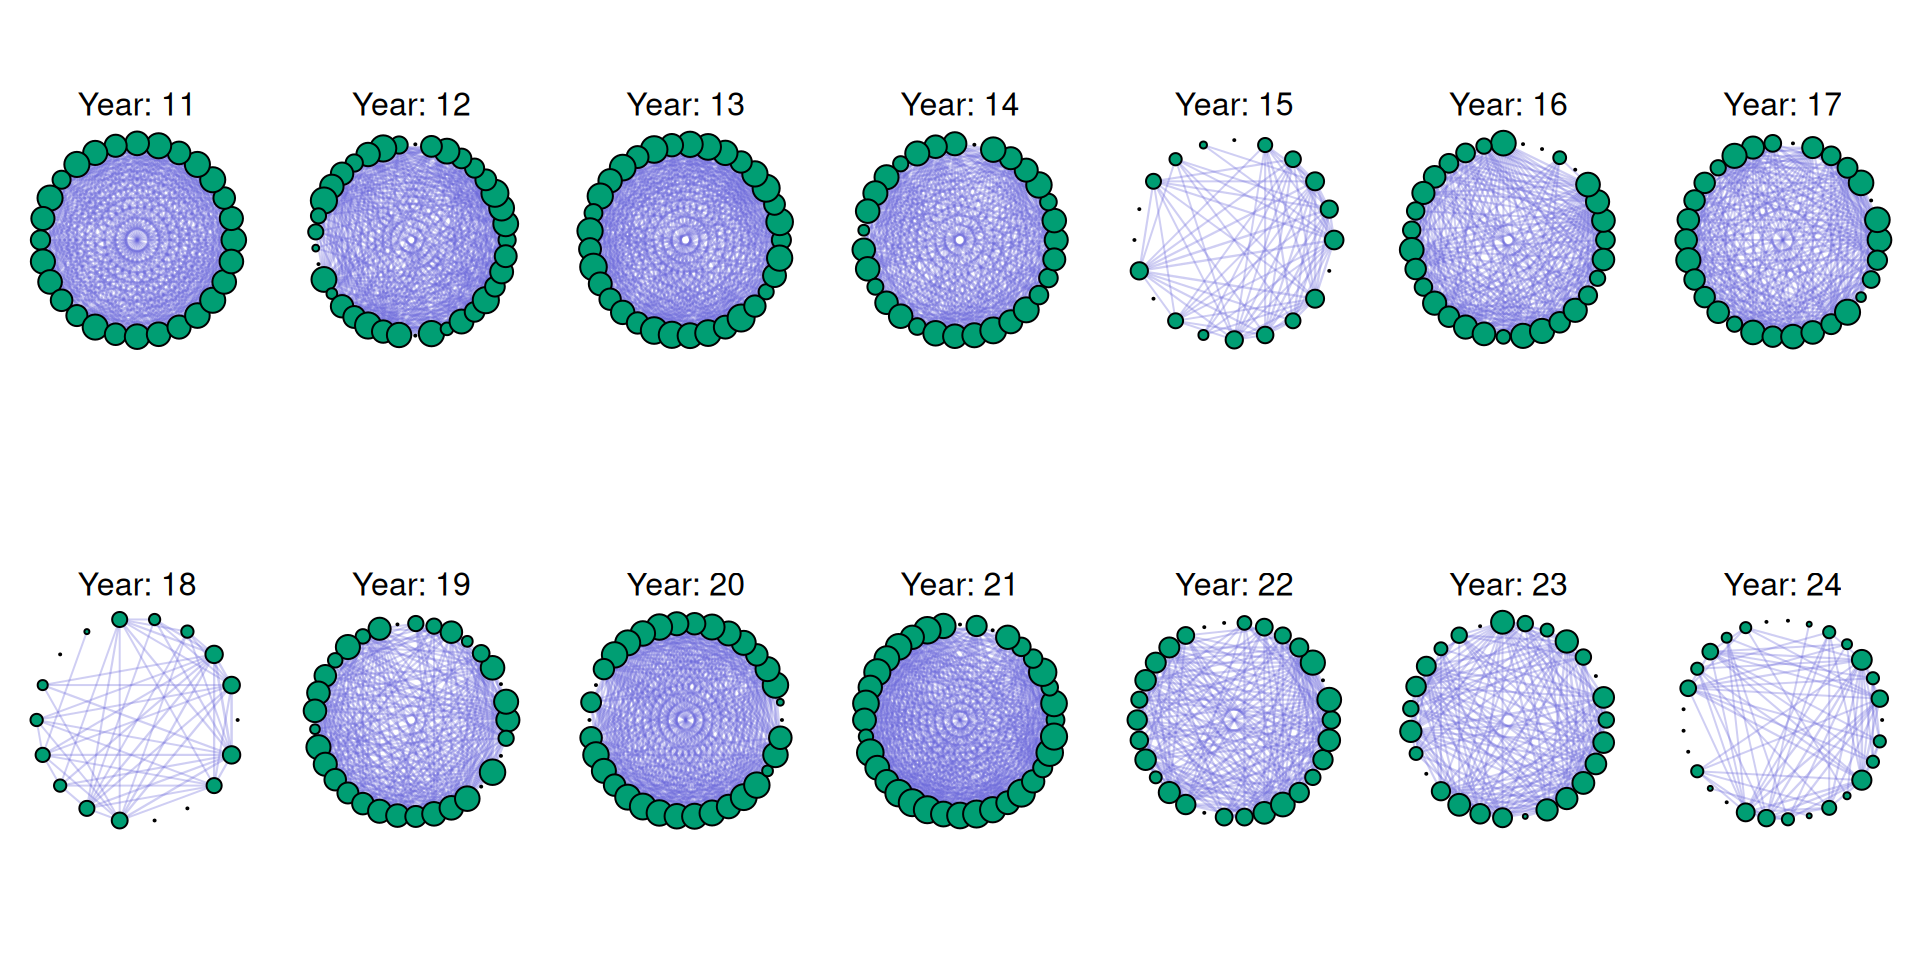
\includegraphics[keepaspectratio]{images/annual_variation.png}}
\end{center}
\end{minipage}%
%
\begin{minipage}{0.05\linewidth}
\end{minipage}%

\end{figure}%
\end{block}

\begin{block}{Diurnal variation in pollinator sharing}
\phantomsection\label{diurnal-variation-in-pollinator-sharing}
\begin{figure}

\begin{minipage}{0.95\linewidth}
\begin{center}
\pandocbounded{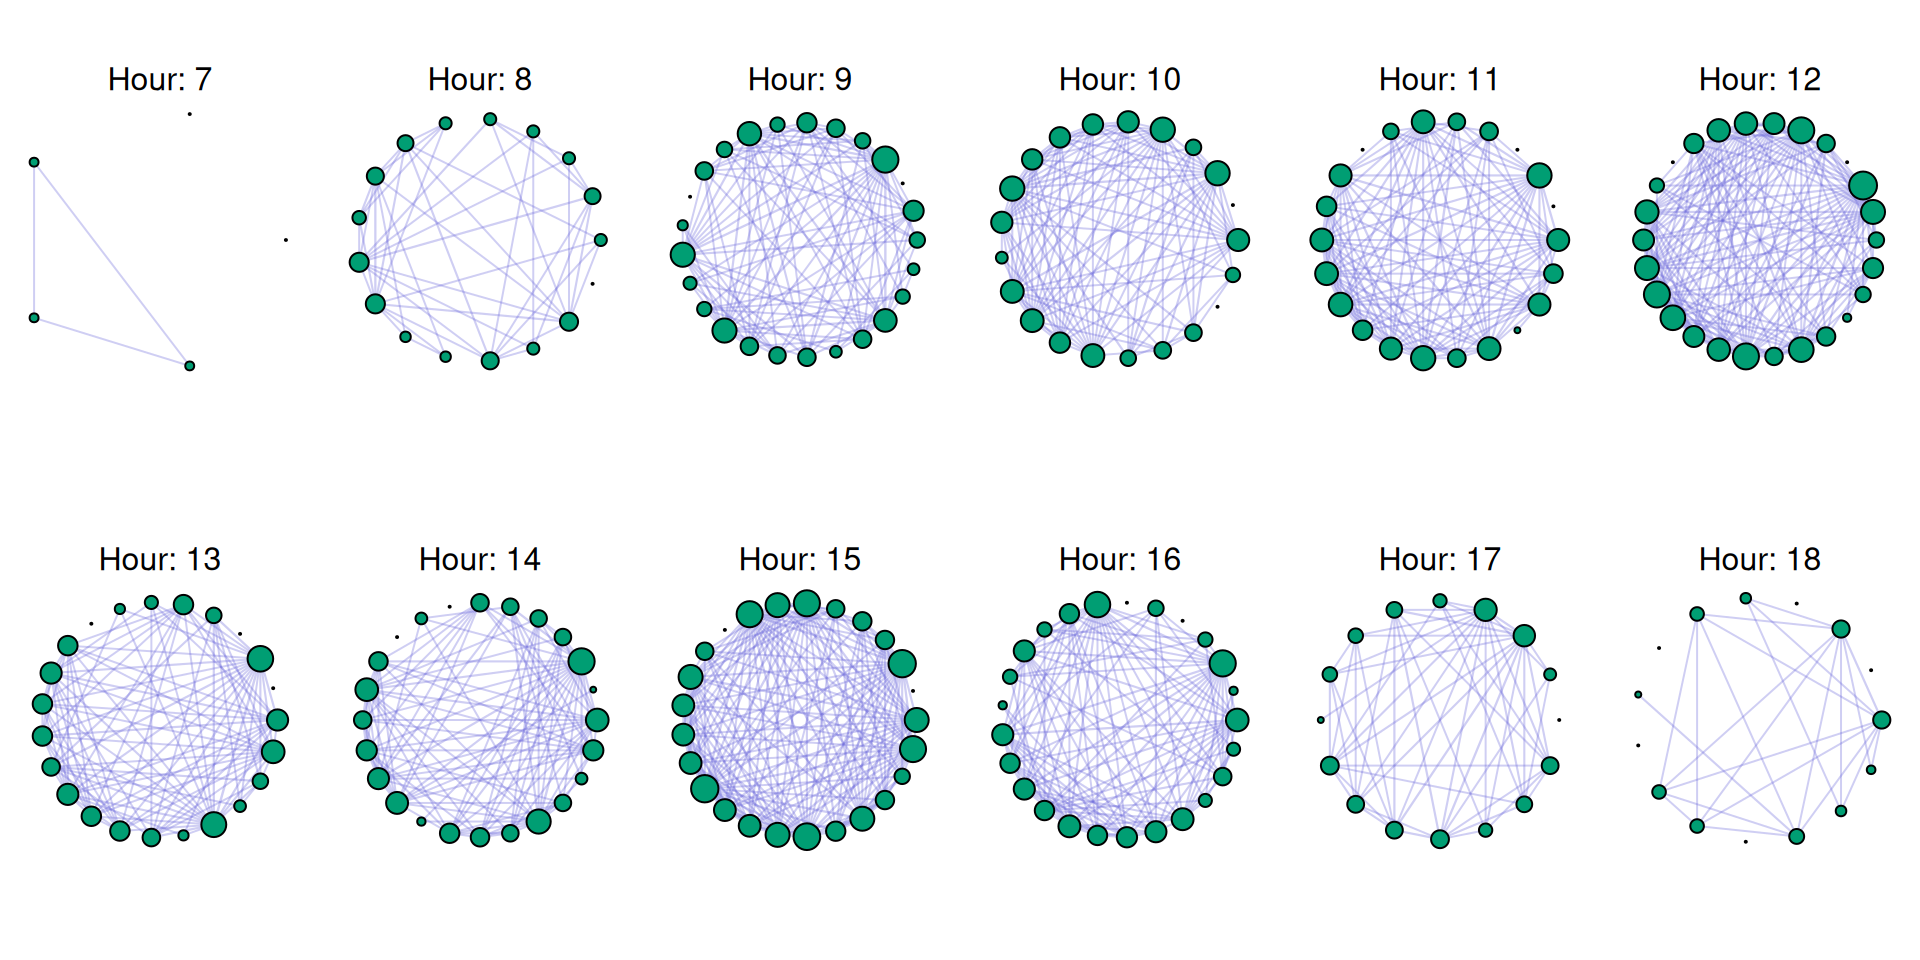
\includegraphics[keepaspectratio]{images/diurnal_variation.png}}
\end{center}
\end{minipage}%
%
\begin{minipage}{0.05\linewidth}
\end{minipage}%

\end{figure}%
\end{block}

\begin{block}{Pollen availability during the day}
\phantomsection\label{pollen-availability-during-the-day}
\begin{figure}

\begin{minipage}{0.95\linewidth}
\begin{center}
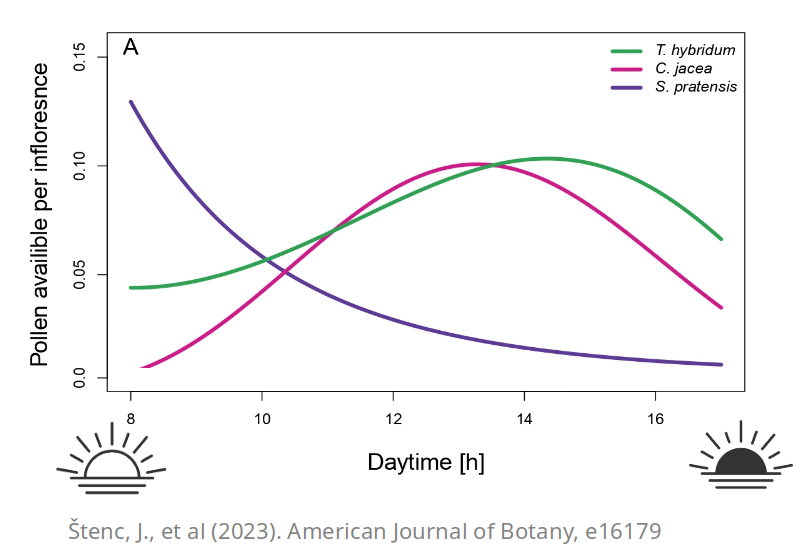
\includegraphics[width=3.78125in,height=\textheight,keepaspectratio]{images/pollen_pres.png}
\end{center}
\end{minipage}%
%
\begin{minipage}{0.05\linewidth}

\end{minipage}%

\end{figure}%
\end{block}

\begin{block}{Pollen transfer during the day}
\phantomsection\label{pollen-transfer-during-the-day}
\begin{center}
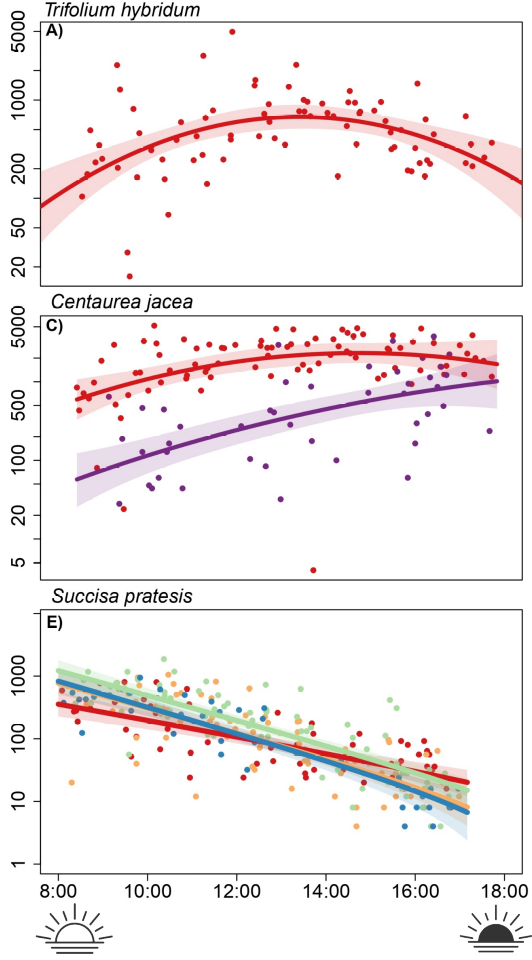
\includegraphics[width=1.44792in,height=\textheight,keepaspectratio]{images/pollen_tra.png}
\end{center}
\end{block}

\begin{block}{Pollen deposition}
\phantomsection\label{pollen-deposition}
\begin{center}
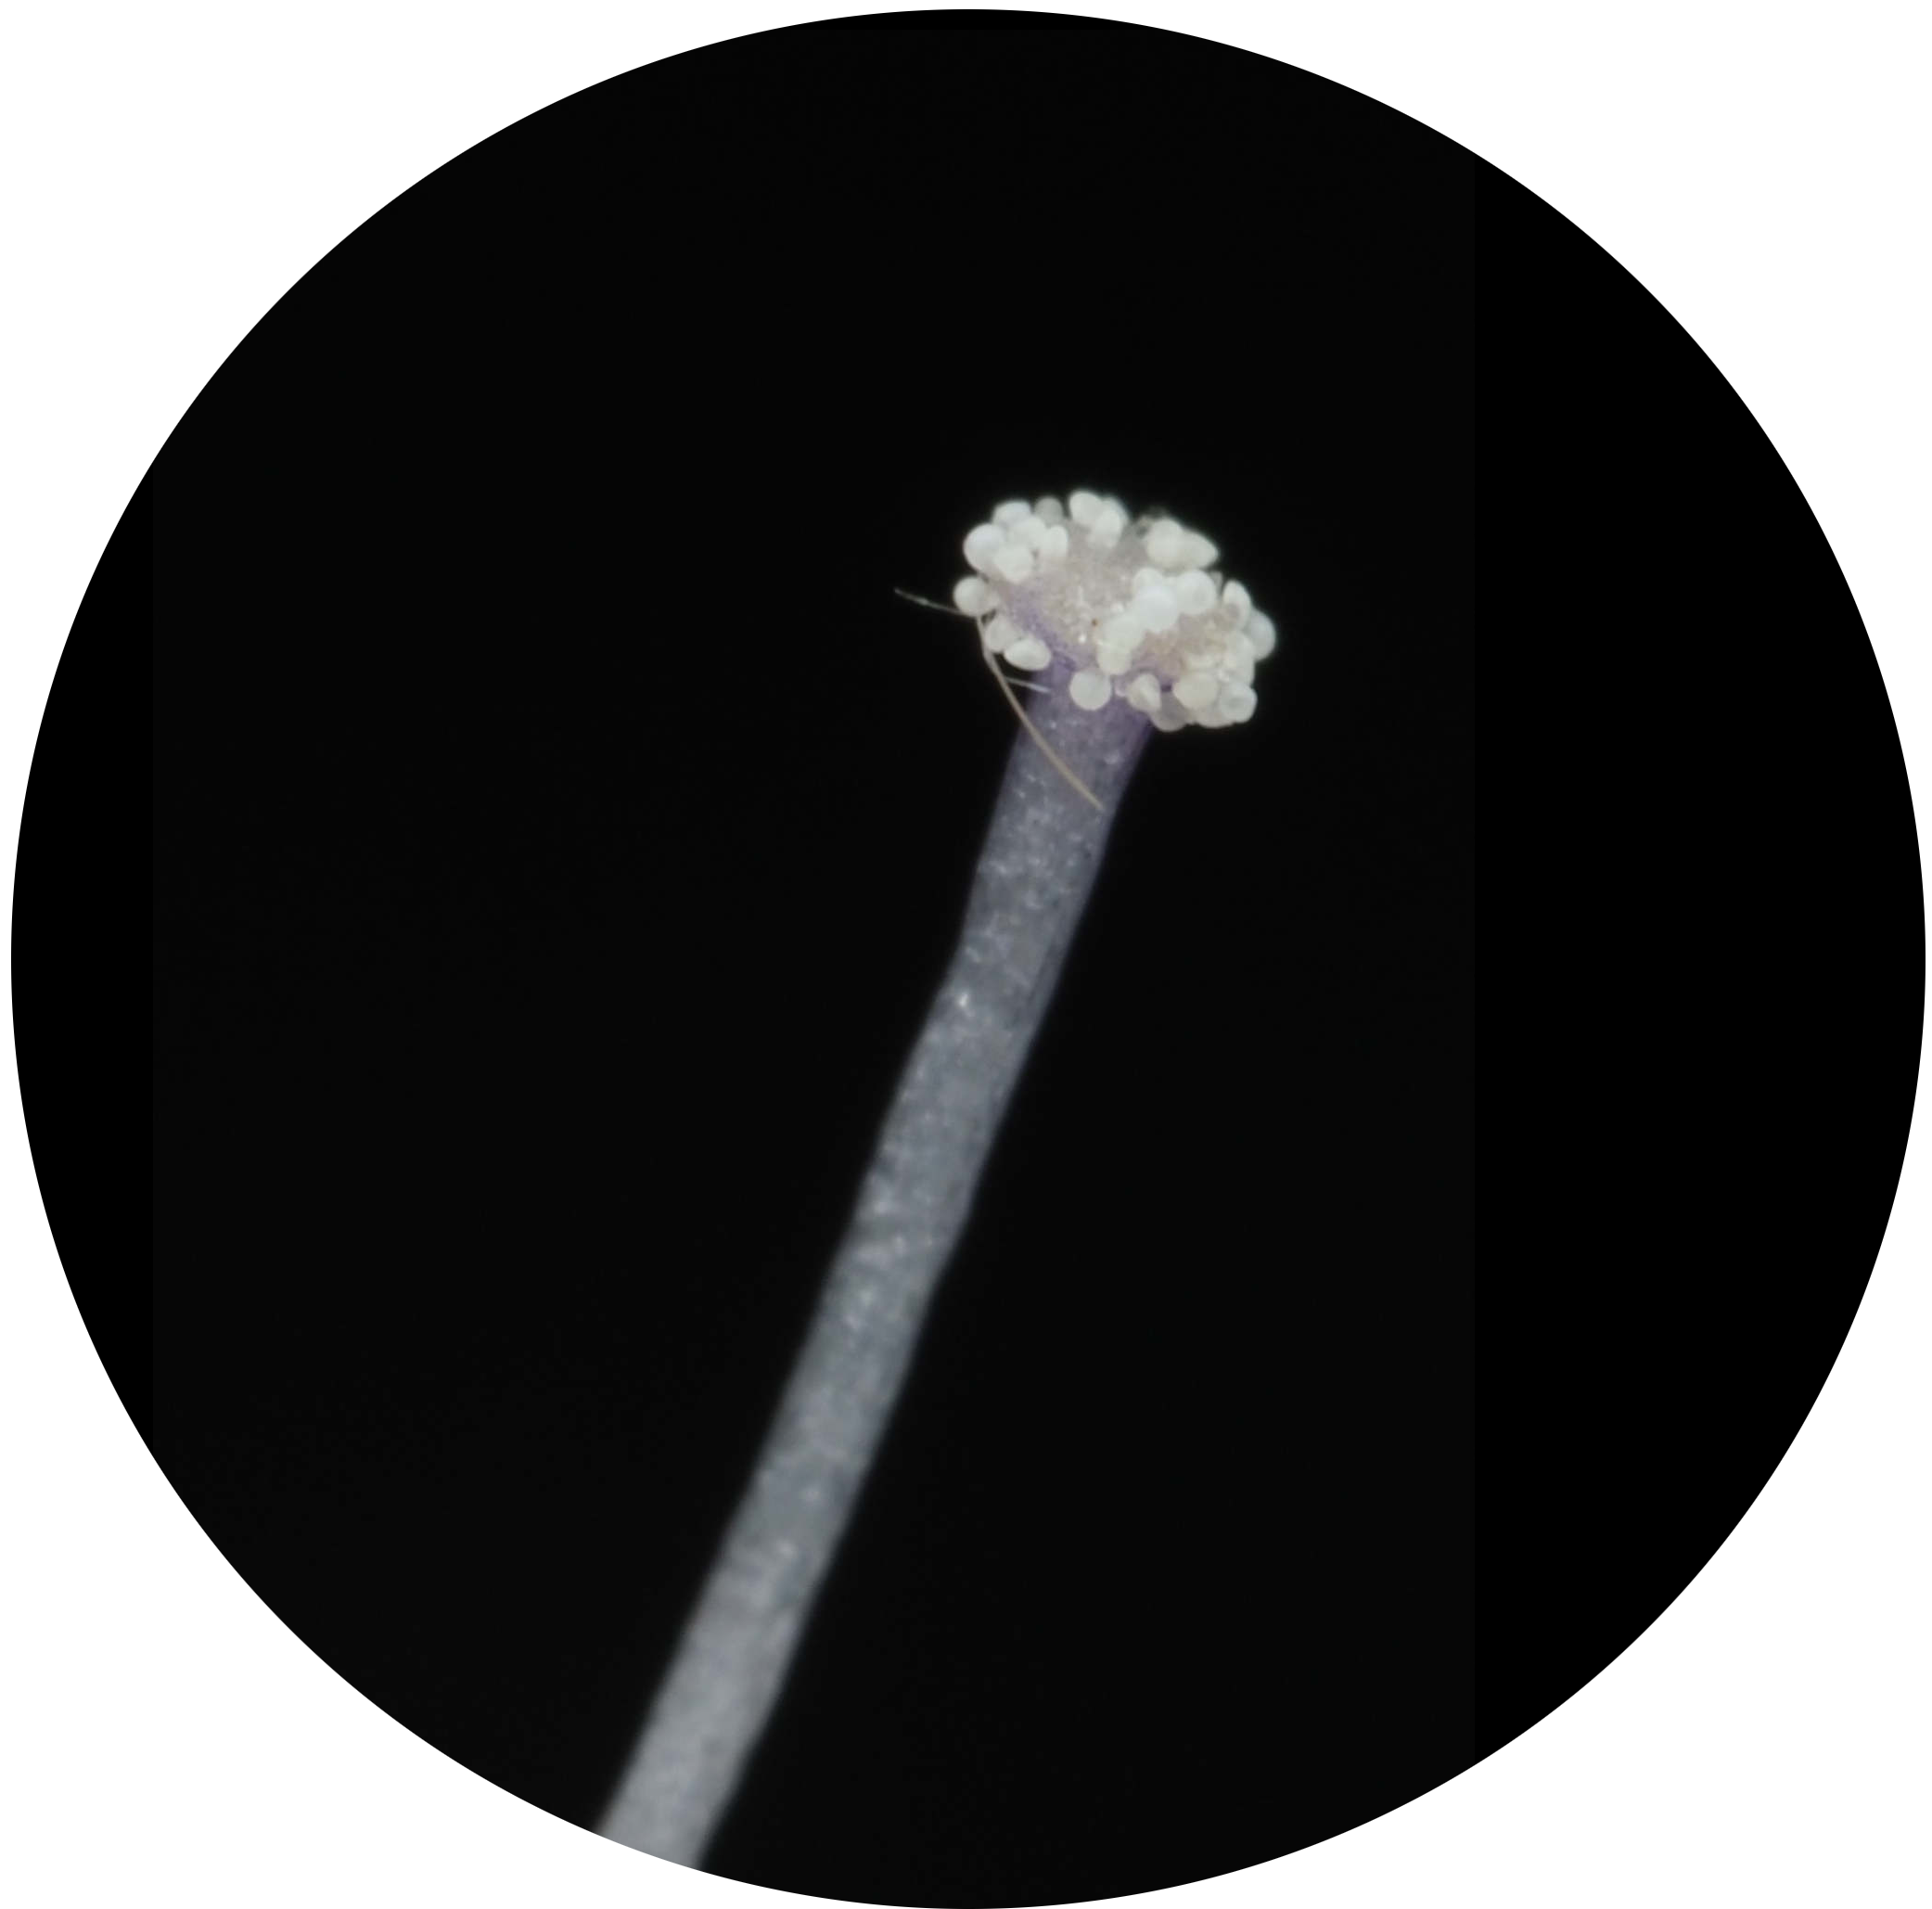
\includegraphics[width=2.53125in,height=\textheight,keepaspectratio]{images/stigma.png}
\end{center}
\end{block}

\begin{block}{Pollen deposition}
\phantomsection\label{pollen-deposition-1}
\begin{center}
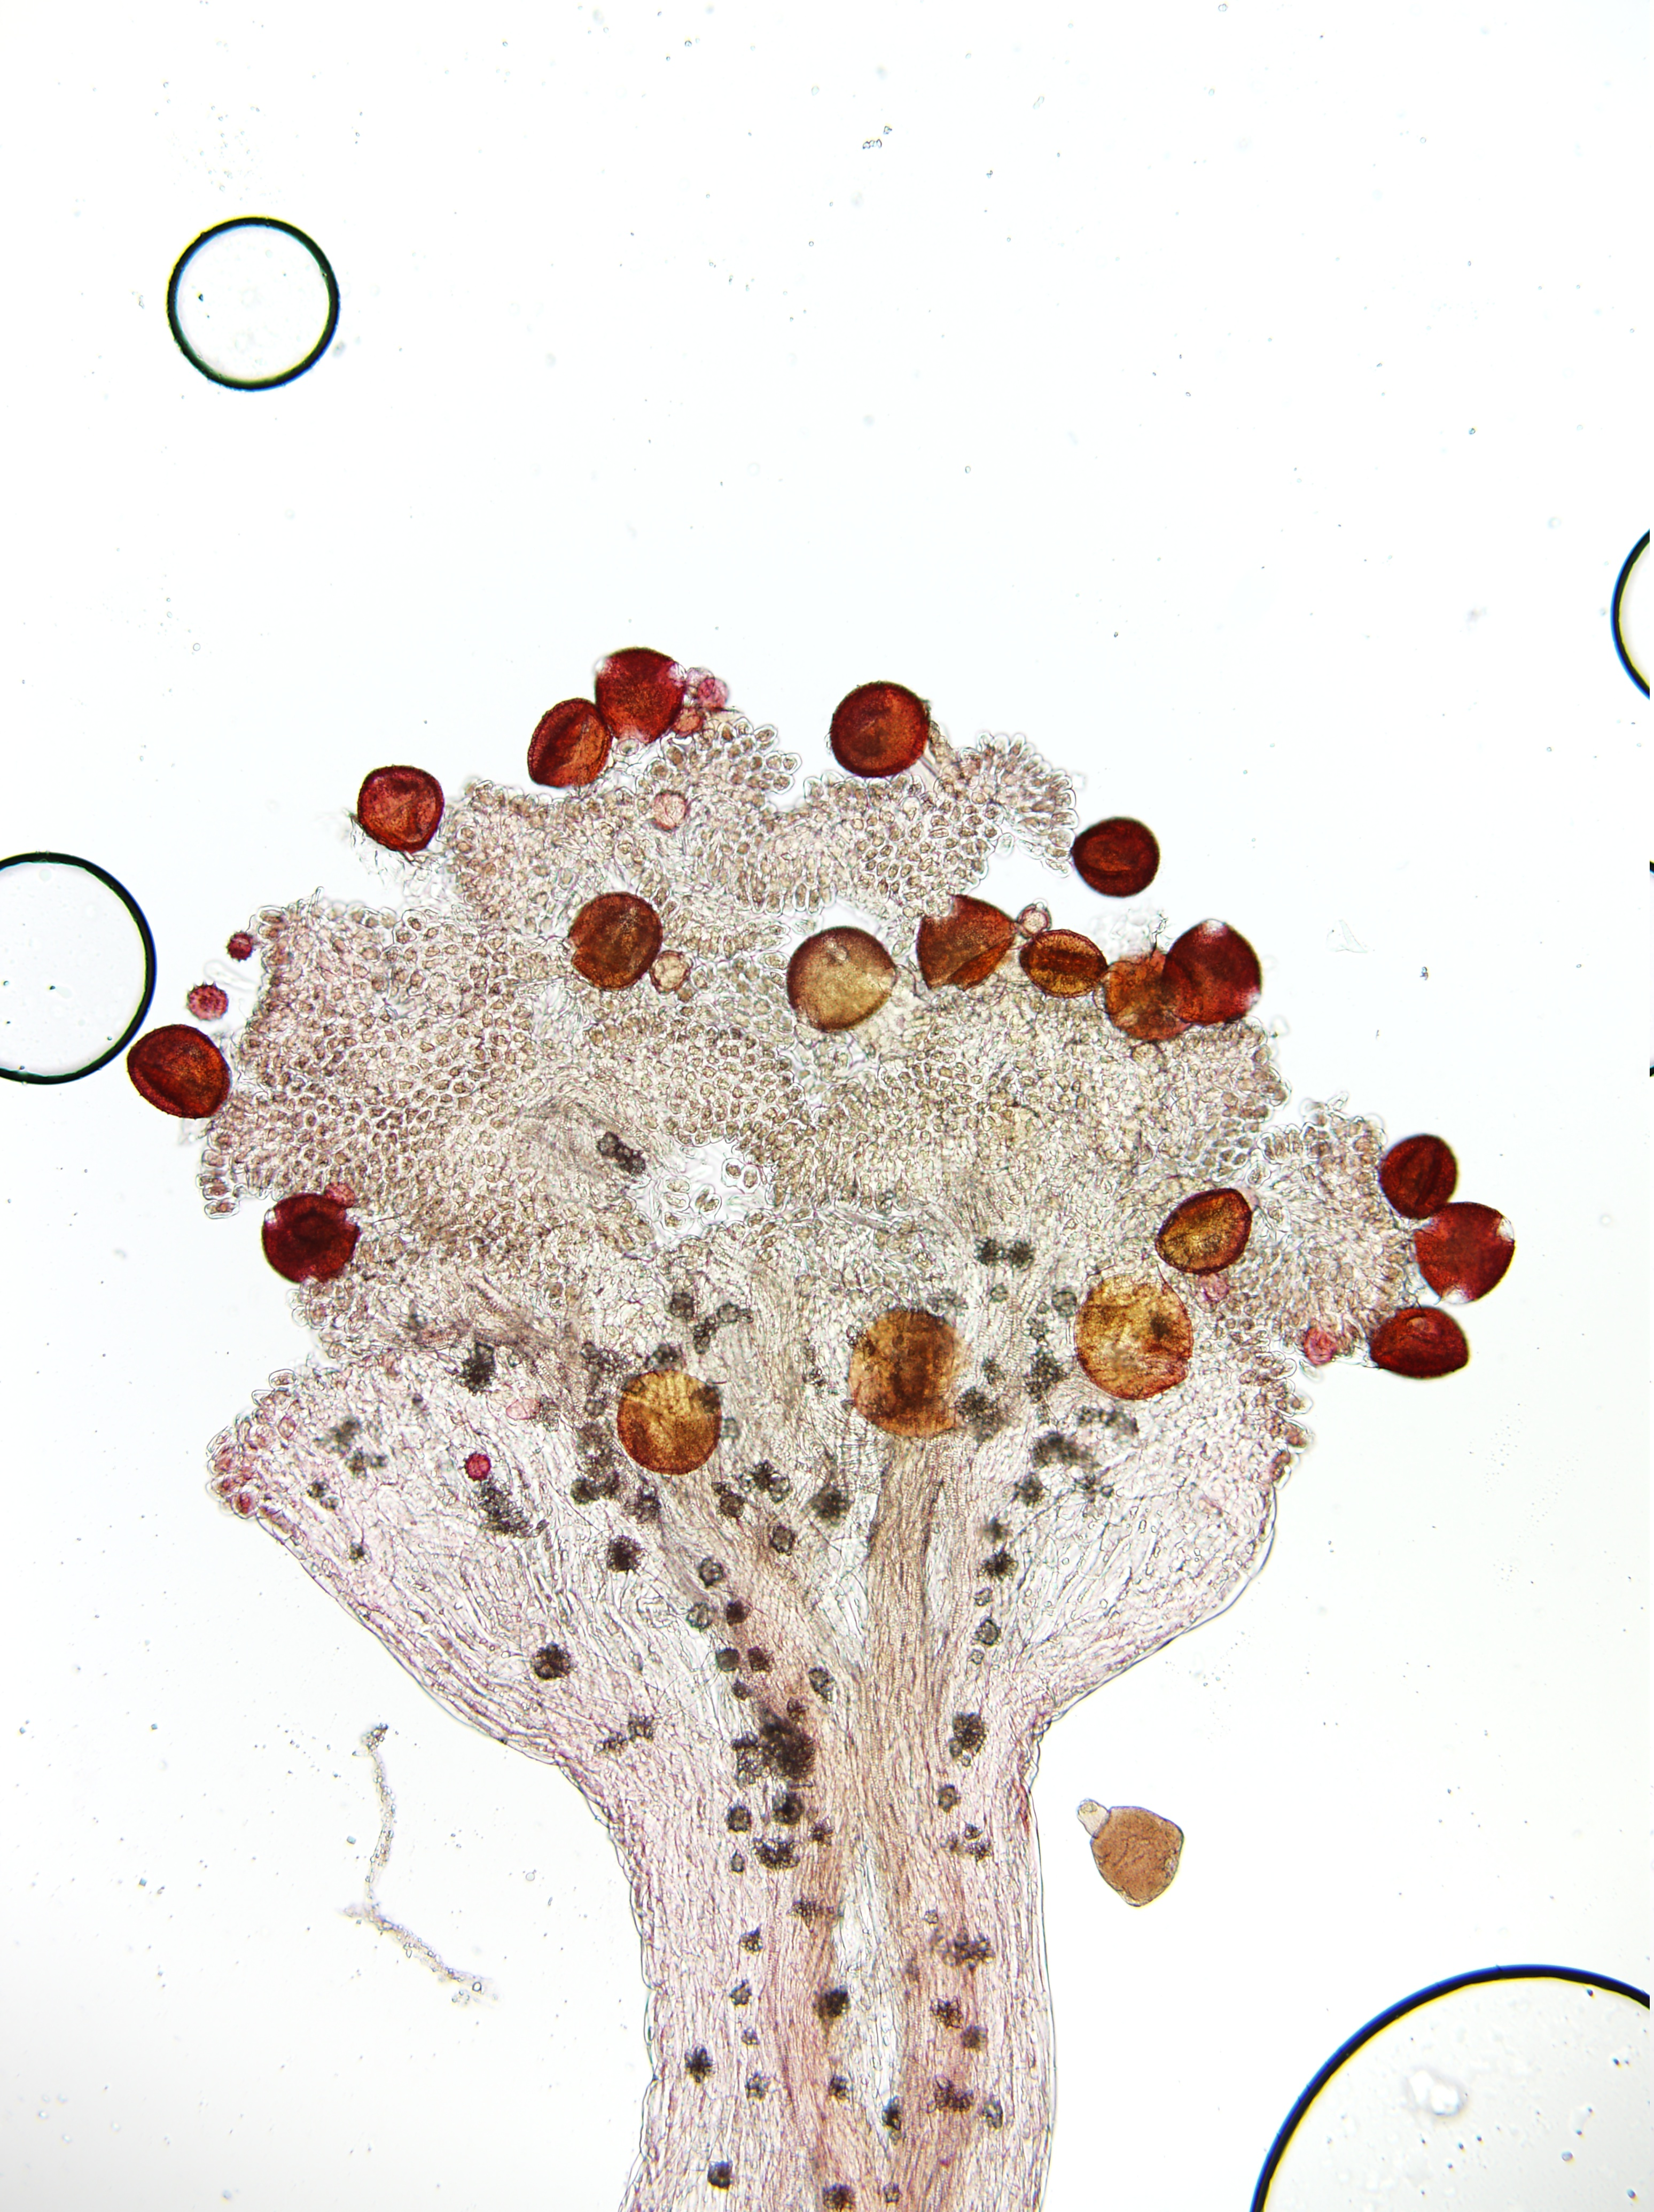
\includegraphics[width=1.94792in,height=\textheight,keepaspectratio]{images/Blizna_Suc_pra_2.jpg}
\end{center}
\end{block}

\begin{block}{Interannual dynamics - Questions}
\phantomsection\label{interannual-dynamics---questions}
\begin{itemize}
\item
  Is pollinator sharing between pairs of plant species stable over
  years?
\item
  Which pair of plants are stable and which ones are variable over
  years?
\item
  Can we identify stable modules within the network?
\item
  How much is pollinator sharing driven by changes in plant abundances
  and how much by other factors (which ones?)
\end{itemize}
\end{block}

\begin{block}{Pollen deposition - questions}
\phantomsection\label{pollen-deposition---questions}
\begin{itemize}
\item
  Does longer exposition of stigma leads to higher deposition than
  necessary for seed development?
\item
  Can longevity serve as mechanism to allow accumulation of pollen?
\item
  Does longer exposition leads to higher proportion of HP?
\end{itemize}
\end{block}

\begin{block}{Progress?}
\phantomsection\label{progress}
So far not so much
\end{block}

\begin{block}{The plan}
\phantomsection\label{the-plan}
\begin{figure}

\begin{minipage}{0.95\linewidth}

\end{minipage}%

\end{figure}%

\begin{itemize}
\item
  
\includegraphics[width=0.3125in,height=\textheight,keepaspectratio]{images/clipboard-2969939425.png}
  - to clean the data and prepare the data sets for analysis (in
  progress)
\item
  
\includegraphics[width=0.3125in,height=\textheight,keepaspectratio]{images/clipboard-3558150951.png}
  - make a package for repeated analyses
\item
  
\includegraphics[width=0.3125in,height=\textheight,keepaspectratio]{images/clipboard-229370691.png}
  - analyse the stability of pollinator sharing
\item
  
\includegraphics[width=0.3125in,height=\textheight,keepaspectratio]{images/clipboard-2272430511.png}
  - write down the MS - draft around Christmass
\end{itemize}
\end{block}

\begin{block}{Data cleaning

\includegraphics[width=0.20833in,height=\textheight,keepaspectratio]{images/clipboard-2969939425.png}}
\phantomsection\label{data-cleaning}
\begin{itemize}
\item
  Plant abundances - now facing the cleaning and decision-making
\item
  Plant-pollinator interactions - 29th of September another meeting
  (11\% to be solved)
\item
  Support data - coordinates, climatic data, traits data
\end{itemize}
\end{block}

\begin{block}{HanPolNet package

\includegraphics[width=0.20833in,height=\textheight,keepaspectratio]{images/clipboard-3558150951.png}}
\phantomsection\label{hanpolnet-package}
\begin{itemize}
\item
  One package to rule all the data - including support data
\item
  Fully available at Github
  \href{https://github.com/Pollination-Ecology-Group/HanPolNet}{
\includegraphics[width=0.3125in,height=\textheight,keepaspectratio]{images/clipboard-4080856661.png}}
\item
  First step: the structure
\item
  I started yesterday
\end{itemize}
\end{block}

\begin{block}{Analysis

\includegraphics[width=0.20833in,height=\textheight,keepaspectratio]{images/clipboard-229370691.png}}
\phantomsection\label{analysis}
\begin{center}

\includegraphics[width=2.08333in,height=\textheight,keepaspectratio]{images/clipboard-4279740602.png}
\end{center}
\end{block}

\begin{block}{Analysis

\includegraphics[width=0.20833in,height=\textheight,keepaspectratio]{images/clipboard-229370691.png}}
\phantomsection\label{analysis-1}
\begin{itemize}
\item
  Interested in seeing stability of

  \begin{itemize}
  \item
    plant species abundance
  \item
    plant distribution patterns
  \item
    plant-pollinator interactions
  \item
    pollinator sharing between plant species
  \end{itemize}
\end{itemize}
\end{block}

\begin{block}{SCAPE 2025}
\phantomsection\label{scape-2025}
\begin{figure}

\begin{minipage}{0.50\linewidth}

\begin{itemize}
\item
  data for pollinator sharing of one plant species
\item
  Data for pollen transfer to that one species from others
\item
  Developing the idea on it
\item
  Using it to test my package functionality
\end{itemize}

\end{minipage}%
%
\begin{minipage}{0.50\linewidth}
\begin{center}
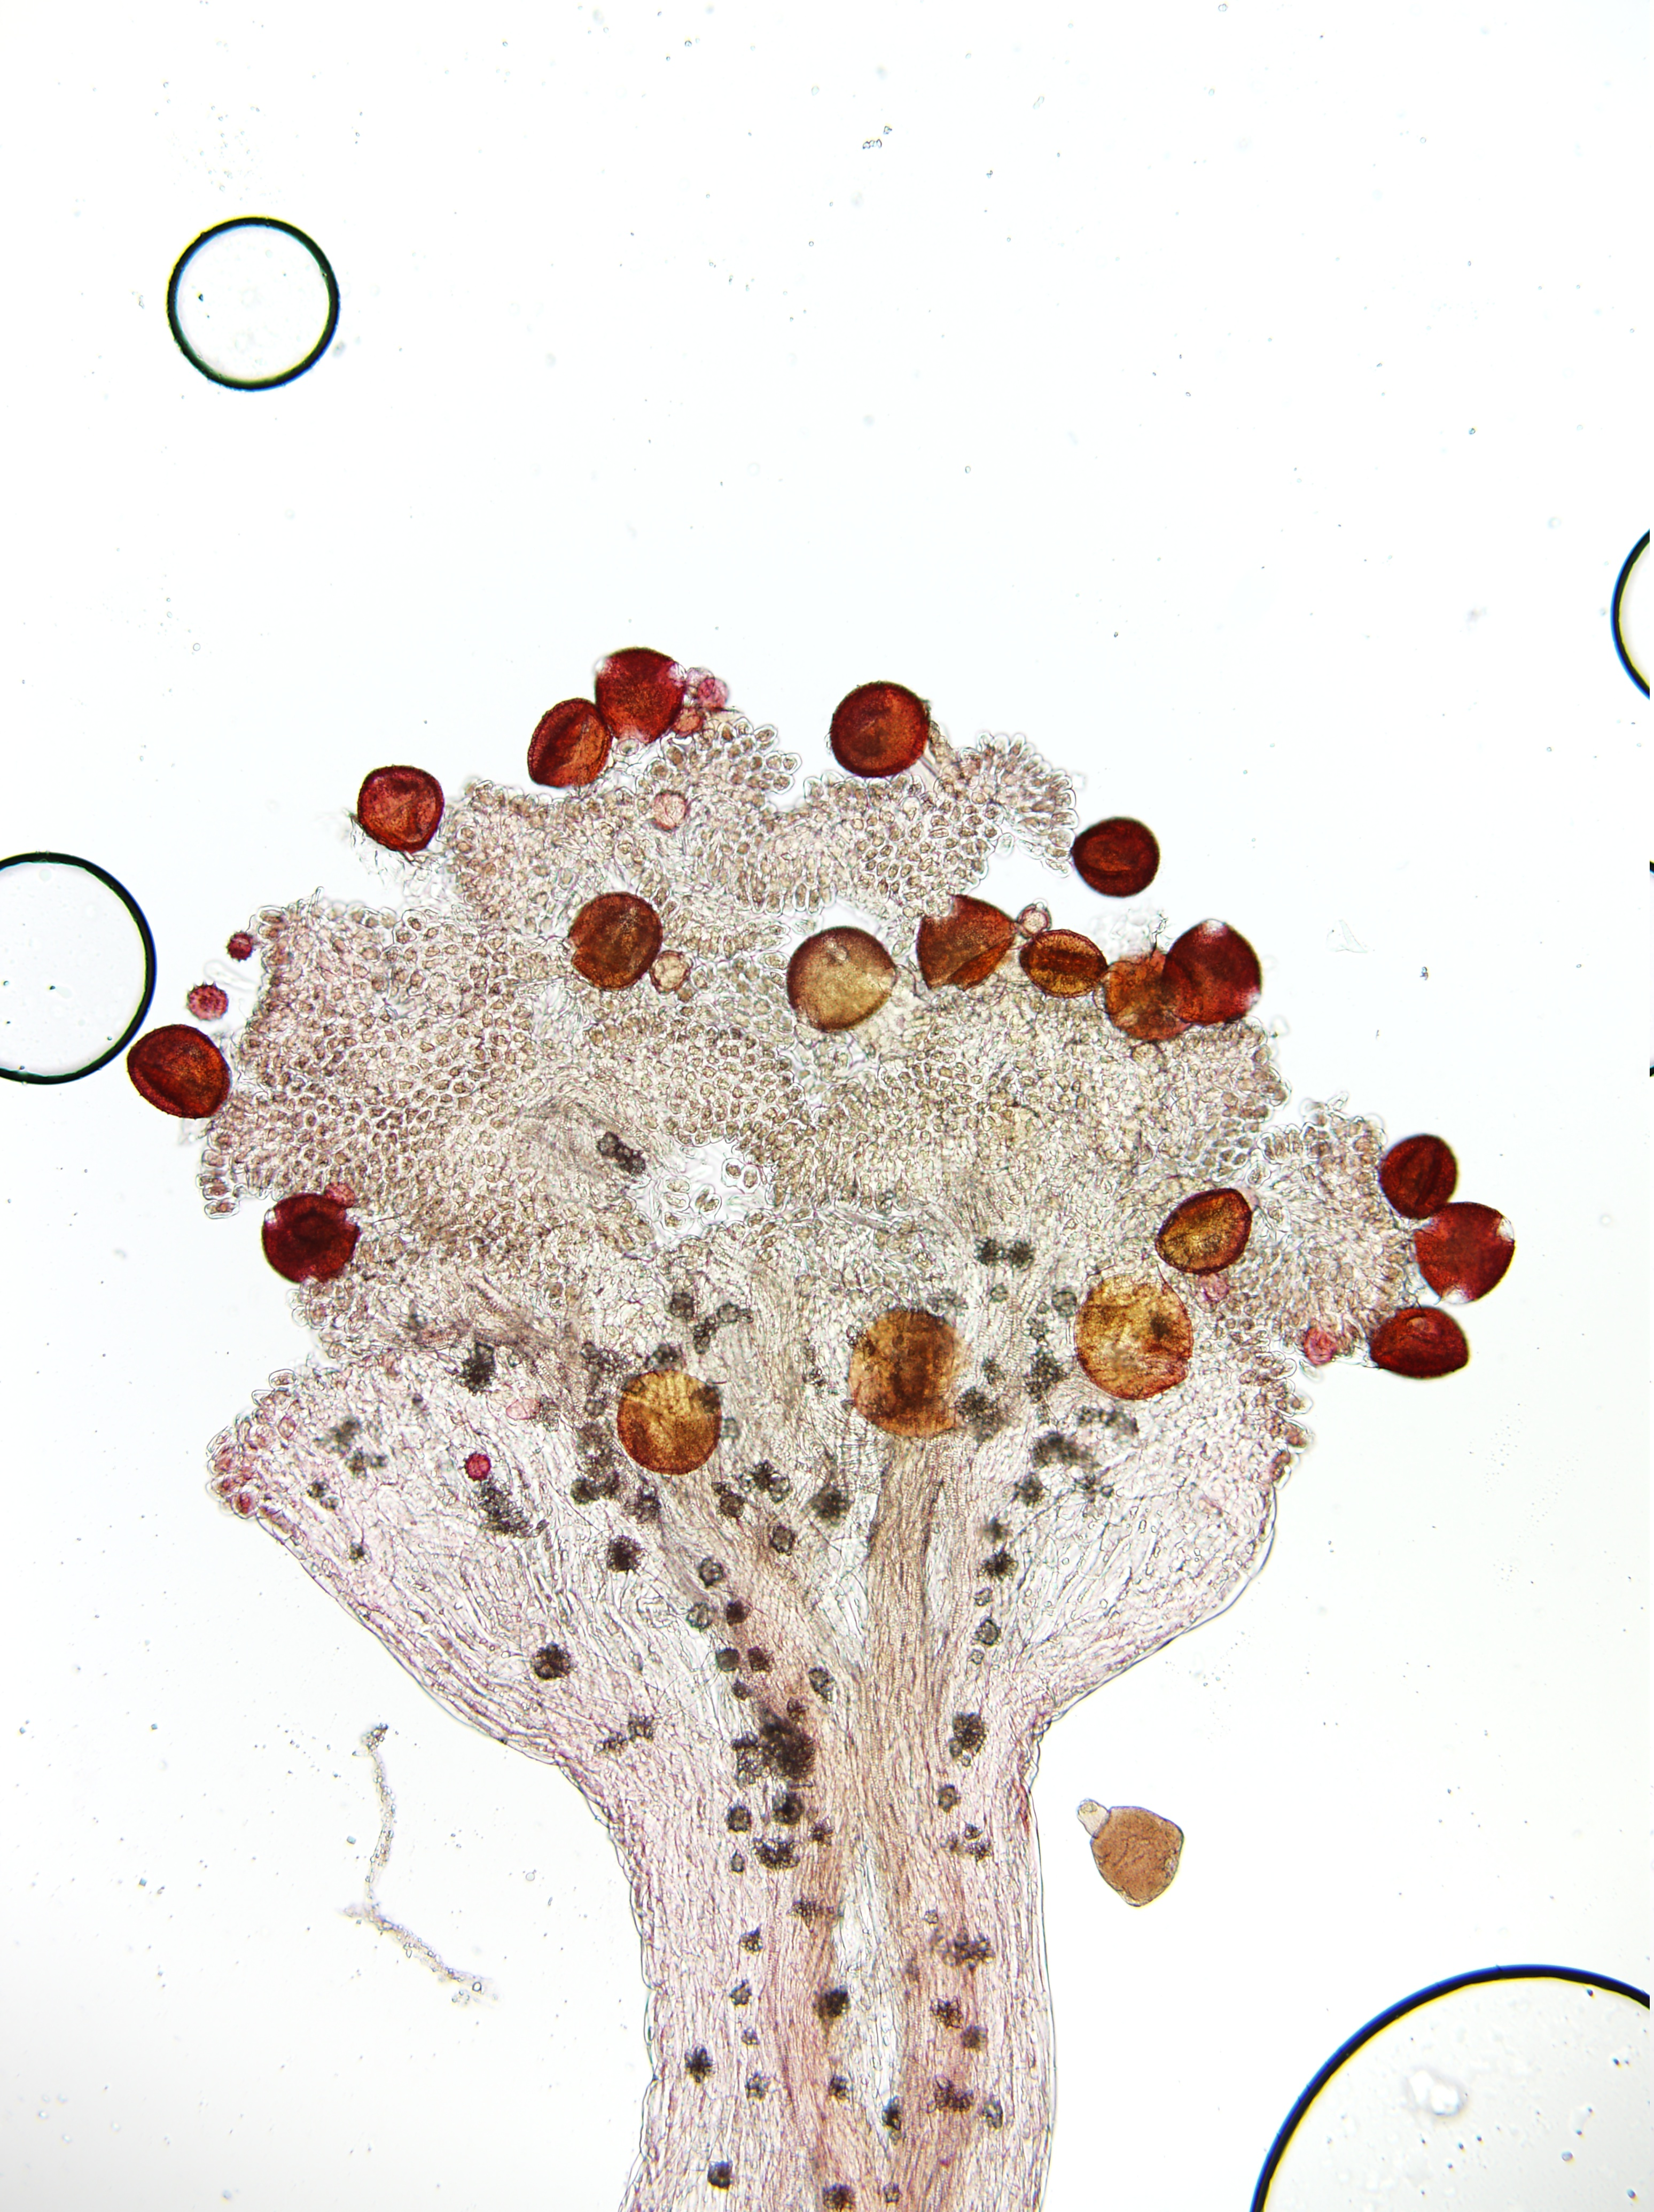
\includegraphics[width=1.5625in,height=\textheight,keepaspectratio]{images/Blizna_Suc_pra_2.jpg}
\end{center}
\end{minipage}%

\end{figure}%
\end{block}
\end{frame}




\end{document}
